% Options for packages loaded elsewhere
\PassOptionsToPackage{unicode}{hyperref}
\PassOptionsToPackage{hyphens}{url}
\PassOptionsToPackage{dvipsnames,svgnames,x11names}{xcolor}
%
\documentclass[
  10pt,
  a4paper,
]{book}
\usepackage{amsmath,amssymb}
\usepackage{iftex}
\ifPDFTeX
  \usepackage[T1]{fontenc}
  \usepackage[utf8]{inputenc}
  \usepackage{textcomp} % provide euro and other symbols
\else % if luatex or xetex
  \usepackage{unicode-math} % this also loads fontspec
  \defaultfontfeatures{Scale=MatchLowercase}
  \defaultfontfeatures[\rmfamily]{Ligatures=TeX,Scale=1}
\fi
\usepackage[]{mathpazo}
\ifPDFTeX\else
  % xetex/luatex font selection
\fi
% Use upquote if available, for straight quotes in verbatim environments
\IfFileExists{upquote.sty}{\usepackage{upquote}}{}
\IfFileExists{microtype.sty}{% use microtype if available
  \usepackage[]{microtype}
  \UseMicrotypeSet[protrusion]{basicmath} % disable protrusion for tt fonts
}{}
\makeatletter
\@ifundefined{KOMAClassName}{% if non-KOMA class
  \IfFileExists{parskip.sty}{%
    \usepackage{parskip}
  }{% else
    \setlength{\parindent}{0pt}
    \setlength{\parskip}{6pt plus 2pt minus 1pt}}
}{% if KOMA class
  \KOMAoptions{parskip=half}}
\makeatother
\usepackage{xcolor}
\usepackage[margin=0.65in]{geometry}
\usepackage{longtable,booktabs,array}
\usepackage{calc} % for calculating minipage widths
% Correct order of tables after \paragraph or \subparagraph
\usepackage{etoolbox}
\makeatletter
\patchcmd\longtable{\par}{\if@noskipsec\mbox{}\fi\par}{}{}
\makeatother
% Allow footnotes in longtable head/foot
\IfFileExists{footnotehyper.sty}{\usepackage{footnotehyper}}{\usepackage{footnote}}
\makesavenoteenv{longtable}
\usepackage{graphicx}
\makeatletter
\newsavebox\pandoc@box
\newcommand*\pandocbounded[1]{% scales image to fit in text height/width
  \sbox\pandoc@box{#1}%
  \Gscale@div\@tempa{\textheight}{\dimexpr\ht\pandoc@box+\dp\pandoc@box\relax}%
  \Gscale@div\@tempb{\linewidth}{\wd\pandoc@box}%
  \ifdim\@tempb\p@<\@tempa\p@\let\@tempa\@tempb\fi% select the smaller of both
  \ifdim\@tempa\p@<\p@\scalebox{\@tempa}{\usebox\pandoc@box}%
  \else\usebox{\pandoc@box}%
  \fi%
}
% Set default figure placement to htbp
\def\fps@figure{htbp}
\makeatother
\setlength{\emergencystretch}{3em} % prevent overfull lines
\providecommand{\tightlist}{%
  \setlength{\itemsep}{0pt}\setlength{\parskip}{0pt}}
\setcounter{secnumdepth}{5}
\usepackage[most]{tcolorbox}
\usepackage{titling}
\usepackage{amsmath,amssymb}
\usepackage{amsmath}
\usepackage[mathcal]{eucal}
\usepackage[table]{xcolor}
\usetikzlibrary{fit, backgrounds}
\usepackage{arydshln}
\usepackage{booktabs}
\usepackage{amsthm}
\usepackage{listings}
\usepackage{tikz}
\usetikzlibrary{matrix}
\usepackage{luacode}
\usepackage{pgfplots}
\pgfplotsset{compat=1.18}
\usetikzlibrary{arrows.meta, positioning}
\renewcommand{\contentsname}{Conteúdo}
\renewcommand{\chaptername}{Capítulo}
\renewcommand*\familydefault{\sfdefault}
\pretitle{\begin{center} 
\includegraphics[width=4in,height=2in]{iseg.png}\LARGE\\}
\usepackage{actuarialsymbol}
\usepackage{booktabs}
\usepackage{longtable}
\usepackage{array}
\usepackage{multirow}
\usepackage{wrapfig}
\usepackage{float}
\usepackage{colortbl}
\usepackage{pdflscape}
\usepackage{tabu}
\usepackage{threeparttable}
\usepackage{threeparttablex}
\usepackage[normalem]{ulem}
\usepackage{makecell}
\usepackage{xcolor}
\usepackage{bookmark}
\IfFileExists{xurl.sty}{\usepackage{xurl}}{} % add URL line breaks if available
\urlstyle{same}
\hypersetup{
  pdftitle={Notas de Processos Estocásticos e Aplicações},
  pdfauthor={Nuno M. Brites},
  colorlinks=true,
  linkcolor={blue},
  filecolor={Maroon},
  citecolor={Blue},
  urlcolor={Blue},
  pdfcreator={LaTeX via pandoc}}

\title{Notas de Processos Estocásticos e Aplicações}
\usepackage{etoolbox}
\makeatletter
\providecommand{\subtitle}[1]{% add subtitle to \maketitle
  \apptocmd{\@title}{\par {\large #1 \par}}{}{}
}
\makeatother
\subtitle{Licenciatura em Matemática Aplicada à Economia e Gestão}
\author{Nuno M. Brites}
\date{2025-07-23}

\usepackage{amsthm}
\newtheorem{theorem}{Teorema}[chapter]
\newtheorem{lemma}{Lema}[chapter]
\newtheorem{corollary}{Corolário}[chapter]
\newtheorem{proposition}{Propriedade}[chapter]
\newtheorem{conjecture}{Conjetura}[chapter]
\theoremstyle{definition}
\newtheorem{definition}{Definição}[chapter]
\theoremstyle{definition}
\newtheorem{example}{Exemplo}[chapter]
\theoremstyle{definition}
\newtheorem{exercise}{Exercício}[chapter]
\theoremstyle{definition}
\newtheorem{hypothesis}{Hipótese}[chapter]
\theoremstyle{remark}
\newtheorem*{remark}{Nota }
\newtheorem*{solution}{Solução }
\begin{document}
\maketitle

{
\hypersetup{linkcolor=}
\setcounter{tocdepth}{2}
\tableofcontents
}
\chapter*{}\label{section}
\addcontentsline{toc}{chapter}{}

\begin{center}
\includegraphics[width=0.4\linewidth]{iseg} \end{center}

\(\,\)

\(\,\)

\(\,\)

\(\,\)

Todas as informações relacionadas com esta UC encontram-se no Fénix.

\(\,\)

Todos os erros e omissões são da minha inteira responsabilidade. Caso detete algum erro ou
gralha, muito agradeço que me informe. Sugestões e comentários também serão muito
bem-vindos!

\(\,\)

\textbf{Esta sebenta não substitui o livro principal.}

\(\,\)

Obrigado,

Nuno M. Brites

\href{mailto:nbrites@iseg.ulisboa.pt}{\nolinkurl{nbrites@iseg.ulisboa.pt}}

ISEG, Setembro de 2025

\vfill

\(\,\)

\(\,\)

\(\,\)

\(\,\)

\textbf{Todos os direitos reservados. Nenhuma parte do conteúdo deste sítio pode ser reproduzida
ou distribuída sem a autorização prévia por escrito do autor. Sem autorização prévia por
escrito, não é permitido copiar ou reproduzir o texto, código e imagens.}

2025 \textbar{} Nuno M. Brites \textbar{}
\href{mailto:nbrites@iseg.ulisboa.pt}{\nolinkurl{nbrites@iseg.ulisboa.pt}}

\chapter{Introdução aos processos estocásticos}\label{introduuxe7uxe3o-aos-processos-estocuxe1sticos}

\section{Introdução}\label{introduuxe7uxe3o}

Quando se pretende estudar fenómenos que não têm qualquer evolução, usam-se \textbf{amostras
aleatórias} (repetições de observações i.i.d.'s). Mas, e se estivermos perante \textbf{variáveis
aleatórias} que já se observaram (ou podiam observar) no passado e que poderemos observar
no futuro? Tal ocorre quando pretendemos estudar, por exemplo:

\begin{itemize}
\item
  cotação diária de uma ação na bolsa de valores;
\item
  evolução da taxa de desemprego num dado período;
\item
  número de pessoas que chegam a uma certa fila para serem atendidas;
\item
  evolução da temperatura num local;
\item
  \(\ldots\)
\end{itemize}

Nos casos acima descritos dispomos apenas de uma única observação (chamada \textbf{trajetória}) a
partir da qual se pretende extrair conclusões. Nesta trajetória não existe independência
entre observações. Tipicamente pretendemos fazer:

\begin{itemize}
\item
  previsão de observações futuras;
\item
  identificação do tipo de evolução;
\item
  filtragem (previsão com a ajuda de observações parciais).
\end{itemize}

\(\,\)

\begin{definition}[Processo estocástico]

Um \textbf{processo estocástico} (PE) é uma família de v.a \(\{X_t, ~t \in T\}\), definida sobre o
mesmo espaço de probabilidade \((\Omega, \mathcal{F}, P)\) e assumindo valores num mesmo
espaço mensurável \((E,\mathcal{B})\), onde:

\begin{itemize}
\item
  \(T:\) espaço dos parâmetros (ou do tempo);
\item
  \(\Omega:\) espaço de resultados possíveis;
\item
  \(\mathcal{F}:\) família de acontecimentos;
\item
  \(P:\) medida de probabilidade;
\item
  \(E:\) conjunto (a definir posteriormente);
\item
  \(\mathcal{B}:\) \(\sigma-\)álgebra de Borel definida em \(E\).
\end{itemize}

\end{definition}

\(\,\)

\begin{remark}

A \(\sigma-\)álgebra de Borel definida em \(E\) satisfaz:

\begin{itemize}
\item
  \(E \in \mathcal{B}\) e \(\emptyset \in \mathcal{B}\);
\item
  \(\mathcal{B}\) é fechado relativamente à diferença, isto é,
  \(\forall A \in \mathcal{B}: A^c \in \mathcal{B}\);
\item
  \(\mathcal{B}\) é fechado relativamente à reunião numerável, isto é,
  \(\bigcup\limits_{i=1}^{n} A_i \in \mathcal{B}, ~A_i \in \mathcal{B}, ~i=1,\ldots,n.\)
\end{itemize}

\end{remark}

\(\,\)

\begin{remark}
\leavevmode

\begin{itemize}
\item
  Dado um espaço de probabilidade \((\Omega, \mathcal{F}, P)\) e um conjunto arbitrário \(T\),
  um PE é uma função \(X(t,\omega)\) definida em \(T \times \Omega\), tal que, para cada
  \(t \in T\), \(X_t(\omega)\) é uma v.a..
\item
  O conceito de PE generaliza o de v.a. fazendo-a depender de um parâmetros \(t\) com
  domínio em \(T\). Assim, podemos interpretar um PE como uma família ordenada de v.a.'s.
\item
  Para cada \(\omega_0\) fixo, \(\omega_0 \in \Omega\), \(X(\omega_0,t)\) é uma função não
  aleatória de \(t\). Deste modo, um PE pode identificar-se com um sistema que a cada ponto
  \(\omega \in \Omega\), faz corresponder uma função de parâmetro \(t\). Cada uma dessas
  funções diz-se uma trajetória ou realização do processo \(X\).
\end{itemize}

\end{remark}

\(\,\)

\begin{definition}[Trajetória de um processo estocástico]
Chama-se \textbf{trajetória} ou \textbf{realização} de um processo estocástico \(X\) à coleção
\(\{X_t(\omega), t \in T\}\), \(\forall ~ \omega \in \Omega\).
\end{definition}

\(\,\)

\begin{remark}

Em geral \((E,\mathcal{B})=(\mathbb{R}^n, \mathcal{B}_{\mathbb{R}^n})\), onde:

\begin{itemize}
\item
  \(\mathbb{R}^n:\) conjunto dos possíveis valores do processo \(X_t\);
\item
  \(\mathcal{B}_{\mathbb{R}^n}:\) \(\sigma-\)álgebra dos borelianos de \(\mathbb{R}^n\);
\item
  Se \(n=1\) o PE chama-se processo estocástico univariado;
\item
  Se \(n>1\) o PE chama-se processo estocástico multivariado;
\item
  \(t:\) instante onde é feita a observação ou o período relativo a essa observação;
\item
  Se \(E\) for finito ou infinito numerável então \(X\) é um PE de espaço de estados
  discreto;
\item
  Se \(E=\mathbb{R}\) então \(X\) é um PE de valores reais;
\item
  Se \(T\) for finito ou infinito numerável então \(X\) é um PE de tempo discreto (tipicamente
  \(T=\mathbb{N}_0\) ou \(T=\mathbb{Z}\));
\item
  Se \(T\) for infinito não numerável então \(X\) é um PE de tempo contínuo (tipicamente
  \(T=\mathbb{R}^+_0\) ou \(T=\mathbb{R}\)).
\end{itemize}

\end{remark}

\(\,\)

\begin{exercise}

Para cada um dos seguintes processos estocásticos indique o espaço parâmetro e o espaço de estados:

\begin{enumerate}
\def\labelenumi{(\alph{enumi})}
\item
  Sejam \(X_i\) a quantidade de cerveja pedida pelo \(i-\)ésimo cliente que entrou num bar e \(N(t)\) o número de clientes que chegaram ao bar até ao instante \(t\). O processo estocástico é
  \[Z_t=\sum\limits_{i=1}^{N(t)}X_i, ~t \geq 0,\]
  onde \(Z_t\) representa a quantidade de cerveja pedida até ao instante \(t\).
\item
  Trinta e seis pontos são escolhidos aleatoriamente no Alaska de acordo com alguma distribuição de probabilidade. Centrado em cada um desses pontos é desenhado um círculo de raio aleatório originando assim uma região \(\Delta\) do Alaska. Seja \(X(A)\) o preço do petróleo extraído no solo da região \(A \cap \Delta\). O processo é
  \[(X(B): ~B \subset Alaska).\]
\item
  Um bebé dorme numa de três posições: (i) de barriga para cima com feição radiante; (ii) enrolada na posição fetal; (iii) na posição fetal, chupando o dedo polegar. Seja \(X_t\) a posição de dormir do bebé no instante \(t\). O processo é \((X_t: ~t\geq 0)\).
\item
  Seja \(X_n\) o estado (ligado ou desligado) de uma fotocopiadora de um escritório ao meio-dia do \(n-\)ésimo dia. O processo é \((X_n: ~ n =1, 2, \dots)\).
\end{enumerate}

\end{exercise}

\section{Tipos clássicos de processos estocásticos}\label{tipos-cluxe1ssicos-de-processos-estocuxe1sticos}

\subsection{Processos de incrementos independentes e estacionários}\label{processos-de-incrementos-independentes-e-estacionuxe1rios}

\begin{definition}[Processo com incrementos inpedendentes]
\(\{X_t, t \in T\}\) é um PE com \textbf{incrementos independentes} sse
\[\forall ~n \in \mathbb{N}, \forall ~t_1, \ldots,t_n \in T: ~t_1 <t_2<\ldots<t_n \implies X_{t_2}-X_{t_1}, X_{t_3}-X_{t_2},\ldots,X_{t_n}-X_{t_{n-1}}\]
são v.a.'s mutuamente independentes.
\end{definition}

\(\,\)

\begin{definition}[Processo com incrementos estacionários]
\(\{X_t, t \in T\}\) tem \textbf{incrementos estacionários} sse \(\forall ~s, t \in T, ~s<t,\) a
distribuição de \(X_t-X_s\) depende apenas da amplitude \(t-s\).
\end{definition}

\(\,\)

Do ponto de vista da modelação, a propriedade de independência de incrementos pode ser
postulada para o modelo quando os resultados obtidos em intervalo de tempo disjuntos forem
independentes. Adicionalmente, a propriedade de estacionariedade de incrementos pode ser
postulada para o modelo quando for plausível que a distribuição de resultados em qualquer
intervalo de tempo depende apenas da amplitude desse intervalo.

\(\,\)

\begin{definition}[Processo de incrementos independentes e estacionários]
Dado um PE \(X:=\{X_t, t \in T\}\), onde \(T\) está munido de uma relação de ordem, \(X\) é um PE
de \textbf{incrementos independentes e estacionários} sse tiver incrementos independentes e
incrementos estacionários.
\end{definition}

\(\,\)

\begin{remark}
Num PE com incrementos estacionários, a distribuição de \(X_{t_{1+h}}-X_{t_1}\) é a mesma de
\(X_{t_{2+h}}-X_{t_2}\), \(\forall ~ t_1,t_2 \in T\) e \(\forall ~ h \in \mathbb{N}\).
\end{remark}

\subsection{Processo estocástico real de 2ª ordem}\label{processo-estocuxe1stico-real-de-2uxaa-ordem}

\begin{definition}[Processo estocástico real de 2ª ordem]

\(\{X_t, t \in T\}\) é um \textbf{PE real de 2ª ordem} sse: \[\forall ~t \in T: E(X_t^2)<+\infty.\]
Usualmente, a caracterização de um PE de 2ª ordem é feita em termos dos dois primeiros
momentos:

\begin{itemize}
\tightlist
\item
  valor médio do processo: \(m(t)=E(X_t), ~\forall ~t \in T\);\\
\item
  covariância do processo: \(\Gamma(s,t)=Cov(X_s,X_t), ~\forall ~s,t \in T\).
\end{itemize}

\end{definition}

\subsubsection{Exemplos de PEs de 2ª ordem}\label{exemplos-de-pes-de-2uxaa-ordem}

\begin{example}[Ruído Branco]

Chama-se \textbf{Ruído Branco} a um PE \(\{\varepsilon_t, ~t \in T\}\) que satisfaz:

\begin{itemize}
\tightlist
\item
  \(\forall ~t \in T, ~E(\varepsilon_t)=0\);\\
\item
  \(\forall ~t \in T, ~Var(\varepsilon_t)=\sigma^2\);\\
\item
  \(\forall ~s, t \in T, s \neq t, ~Cov(\varepsilon_s,\varepsilon_t)=0\).
\end{itemize}

\end{example}

\(\,\)

\begin{example}[Processo Gaussiano]
\(\{X_t, t \in T\}\) diz-se um \textbf{Processo Gaussiano} sse:\\
\[\forall ~n \in \mathbb{N}, \forall ~t_1, t_2, \ldots, t_n \in T: (X_{t_1}, X_{t_2}, \ldots, X_{t_n})\]
for um vetor aleatório Gaussiano, isto é,
\[X_{t_i} \sim \mathcal{N}(\mu,\sigma^2), ~\forall ~t_i \in T.\]
\end{example}

\subsection{Processos estacionários}\label{processos-estacionuxe1rios}

\begin{definition}[Processo estacionário em sentido forte]
Um PE \(\{X_t, t \in T\}\) é \textbf{estacionário em sentido forte} (ou fortemente estacionário)
se,
\[\forall ~h \in T, \forall ~n \in \mathbb{N}, \forall ~t_1, \ldots, t_n, ~(t_1 < \ldots < t_n), ~(X_{t_1}, \ldots, X_{t_n}) \,{\buildrel d \over =}\, (X_{t_1+h}, \ldots, X_{t_n+h}),\]
isto é, se a distribuição de \(\{X_t, t \in T\}\) é igual à distribuição de
\((X_{t_1+h}, \ldots, X_{t_n+h})\), \(~\forall ~h \in T\).
\end{definition}

Como consequência da estacionariedade forte, temos o seguinte Teorema:

\begin{theorem}

Se \(\{X_t, t \in T\}\) é um PE de 2ª ordem e se é fortemente estacionário, então:

\begin{itemize}
\item
  \(E(X_t)=m\), isto é, a média do processo é independente de \(t\);
\item
  \(\forall ~h \in T, ~ \Gamma(t,t+h)=Cov(X_t,X_{t+h})=Cov(X_0,X_h)=\gamma(h)\),
  independente de \(t\).
\end{itemize}

\end{theorem}

\(\,\)

\begin{definition}[Processo estacionário em sentido fraco]

Um PE \(\{X_t, t \in T\}\) é \textbf{estacionário em sentido fraco} (ou estacionário de 2ª ordem),
sse:

\begin{itemize}
\item
  \(\forall ~t \in T, ~E(X^2_t)< + \infty\);
\item
  \(\forall ~t \in T, ~E(X_t)=m\), independente de \(t\);
\item
  \(\forall ~t \in T, \forall ~h \in T,  ~Cov(X_t,X_{t+h})=\gamma(h)\), isto é, a covariância
  apenas depende de \(h\).
\end{itemize}

\end{definition}

\(\,\)

\begin{remark}
A função \(\gamma(h), ~\forall ~ h \in T\), chama-se \textbf{função de autocovariância}. Se \(h=0\),
então \(Cov(X_t,X_{t+h})=Var(X_t)=\gamma(0), ~\forall ~t \in T.\) A esta propriedade chama-se
propriedade da homocedasticidade.
\end{remark}

\(\,\)

Vejamos agora que o Ruído Branco, \(\{\varepsilon_t, ~t \in T\}\), é um exemplo de um PE
estacionário de 2ª ordem:

\begin{example}
\leavevmode

\begin{itemize}
\item
  \(E(\varepsilon_t)=0\);
\item
  \(Var(\varepsilon_t)=\sigma^2 \implies E(\varepsilon^2_t) < + \infty\);
\item
  \(t \neq s, ~Cov(\varepsilon_s,\varepsilon_t)=0, \implies\) independência de \(t\) e de \(s\).
\end{itemize}

Assim,

\[
\gamma(h)=
\begin{cases}
\sigma^2, \quad h=0,\\
0, \quad h \neq 0.
\end{cases}
\] Logo, estão satisfeitas as condições de estacionariedade fraca.

\end{example}

\(\,\)

\begin{remark}[Observação importante]
\[\text{Estacionariedade forte} + E(X_t^2) <+\infty \Rightarrow \text{Estacionariedade fraca}.\]
\[\text{Estacionariedade fraca} \nRightarrow \text{Estacionariedade forte}.\]
\end{remark}

\(\,\)

\begin{example}
Considere o PE \((X_t, ~t \in \mathbb{N})\) onde \(X_t\) tem distribuição de Cauchy, isto é, com
f.d.p. \(f(x)=\dfrac{1}{\pi(1+x^2)}\). Uma vez que não existe \(E(X_t)\), então \(E(X_t^2)\) não
está definido. Assim, o processo é fortemente estacionário mas não é fracamente
estacionário.
\end{example}

\(\,\)

\begin{proposition}[Propriedades da função de autocovariância em processos estacionários]

A função de autocovariância \(\gamma(h)\) goza das seguintes propriedades:

\begin{itemize}
\item
  \(\gamma(h)=\gamma(-h), \forall ~h \in \mathbb{Z}\), isto é, a função de autocovariância é
  par;
\item
  \(\forall ~n \in \mathbb{N}, \forall ~a_j \in \mathbb{R}, \forall ~t_j \in \mathbb{Z}, ~j=1, \ldots,n:\)
  \[\sum\limits_{j=1}^{n}\sum\limits_{k=1}^{n} a_ja_k\gamma(t_j-t_k) \geq 0,\] isto é,
  trata-se de uma função semi-definida positiva.
\end{itemize}

\end{proposition}

\(\,\)

\begin{definition}[Função de autocorrelação em processos estacionários]
Seja \(\{X_t, t \in T\}\) um PE estacionário. Chama-se \textbf{função de autocorrelação} à função
\(\rho\) definida por:
\[\rho(h)=Corr(X_t,X_{t+h})=\dfrac{Cov(X_t,X_{t+h})}{\sqrt{V(X_t)}\sqrt{V(X_{t+h})}}=\dfrac{\gamma(h)}{\gamma(0)}.\]
\end{definition}

\(\,\)

\begin{proposition}[Propriedades da função de autocorrelação em processos estacionários]

A função de autocorrelação \(\rho(h)\) goza das seguintes propriedades:

\begin{itemize}
\item
  \(\rho(h)=\rho(-h), \forall ~h \in \mathbb{Z}\), isto é, a função de autocovariância é
  par;
\item
  \(\forall ~n \in \mathbb{N}, \forall ~a_j \in \mathbb{R}, \forall ~t_j \in \mathbb{Z}, ~j=1, \ldots,n:\)
  \[\sum\limits_{j=1}^{n}\sum\limits_{k=1}^{n} a_ja_k\rho(t_j-t_k) \geq 0,\] isto é,
  trata-se de uma função semi-definida positiva.
\end{itemize}

\end{proposition}

\(\,\)

\begin{exercise}

Sejam \(X\) e \(Y\) duas variáveis aleatórias não enviesadas, não correlacionadas e com a mesma variância \(\sigma^2>0\). Considere-se o processo estaocástico \((Z_t: ~t \in \mathbb{Z})\) definido por:

\[Z_t=f(t) \cdot X + g(t) \cdot Y, \quad t \in \mathbb{Z},\]
onde \(f\) e \(g\) são função deterministas.

\begin{enumerate}
\def\labelenumi{(\alph{enumi})}
\item
  Encontre expressões para \(f\) e \(g\) de modo a garantir que o processo \((Z_t: ~t \in \mathbb{Z})\) admita variância constante mas não seja necessariamente estacionário em sentido fraco.
\item
  Concretize \(f\) e \(g\) de modo a que \((Z_t: ~t \in \mathbb{Z})\) seja fracamente estacionário.
\end{enumerate}

\end{exercise}

\(\,\)

\begin{exercise}

Seja \(\varepsilon = (\varepsilon_t: ~t \in \mathbb{Z})\) um ruído branco de variância \(\sigma^2 > 0\). Considere os processos estocásticos \(X = (X_t: ~ t \in \mathbb{Z})\) e \(Y = (Y_t: ~ t \in \mathbb{Z})\) definidos do seguinte modo:
\[X_t = \varepsilon_t \quad \text{e} \quad Y_t = (-1)^t \varepsilon_t, \quad \forall ~ t \in \mathbb{Z}.\]

\begin{enumerate}
\def\labelenumi{(\alph{enumi})}
\item
  Prove que \(X\) e \(Y\) são fracamente estacionários.
\item
  Mostre que o processo \((Z_t = X_t + Y_t: ~  t \in \mathbb{Z})\) é um processo não estacionário.
\end{enumerate}

\end{exercise}

\(\,\)

\begin{exercise}

Considere um processo estocástico \(Y = (Y_t: t \in \mathbb{Z})\) tal que \(Y_t = \varepsilon_t - \theta \varepsilon_{t-1}\), \(\theta \in [-1,1]\), onde \((\varepsilon_t: t \in \mathbb{Z})\) é um ruído branco gaussiano de variância \(\sigma^2 > 0\).

\begin{enumerate}
\def\labelenumi{(\alph{enumi})}
\item
  Defina processo gaussiano e mostre que \(Y\) é gaussiano.
\item
  Determine a distribuição da variável aleatória \(Y_t, ~\forall ~t \in \mathbb{Z}\).
\item
  Determine a função de autocorrelação de \(Y\).
\item
  O que pode concluir quanto à estacionariedade forte e fraca de \(Y\)?
\end{enumerate}

\end{exercise}

\(\,\)

\begin{exercise}

Seja \(X = (X_t: ~ t \geq 0)\) um processo estocástico, definido sobre o espaço de probabilidade \((\Omega, \mathcal{F}, P)\), tal que, para todo \(t \geq 0\), \(X_t \sim \mathcal{N}(0, t)\), e \(P(X_0 = 0) = 1\).

\begin{enumerate}
\def\labelenumi{(\alph{enumi})}
\item
  Diga em que condições será \(X\) um processo de incrementos independentes e estacionários.
\item
  Supondo que \(X\) é um processo de incrementos independentes e estacionários, mostre que: (i) \(\forall~ t, s \in [0,+\infty[\), com \(t > s\), tem-se que \(X_t - X_s \sim \mathcal{N}(0, |t - s|)\); (ii) \(X\) é um processo gaussiano centrado.
\item
  Considere o processo estocástico \(Y = (Y_t: t \geq 0)\) tal que:
  \[
  Y(t)= 
  \begin{cases}
  t, & X_t \geq 0\\
  -t, & X_t < 0.\\
  \end{cases}
  \]
  Mostre que \(Y\) é um processo estocástico de segunda ordem centrado. Será \(Y\) estacionário em algum sentido? Justifique.
\end{enumerate}

\end{exercise}

\(\,\)

\begin{exercise}

Sejam \(X = (X_t: ~t \in \mathbb{Z})\) e \((\varepsilon_t: ~t \in \mathbb{Z})\) dois processos estocásticos definidos sobre o espaço de probabilidade \((\Omega, \mathcal{F}, P)\), tais que:
\[
\forall ~t \in \mathbb{Z}, \quad X_t = \sum\limits_{j=0}^{+\infty} \left( \frac{4}{5} \right)^j \varepsilon_{t-j}.
\]

\begin{enumerate}
\def\labelenumi{(\alph{enumi})}
\item
  Explique em que condições será \(\varepsilon\) um ruído branco.
\item
  Suponha que \(\varepsilon\) é um ruído branco tal que \(E[\varepsilon_t^2] = 9/50\). (i) Prove que \(X\) é fracamente estacionário e indique as respetivas função média e função de autocovariância; (ii) Suponha agora que \(X\) é um processo gaussiano. Indique a distibuição do vector aleatório \((X_t, X_s), ~ \forall ~ t, s \in \mathbb{Z}\).
\item
  Considere o processo estocástico \(Y = (Y_t: t \in \mathbb{Z})\) tal que:
  \[
  Y_t = 
  \begin{cases}
  1/2, & X_t \geq 0 \\
  -1, & X_t < 0,
  \end{cases}
  \]
  admitindo que \(X\) está nas condições da alínea b) ii). Calcule a função média de \(Y\) e mostre que \(Y\) é fracamente estacionário.
\end{enumerate}

\end{exercise}

\(\,\)

\begin{exercise}

Seja \((\varepsilon_t: t \in \mathbb{Z})\) um ruído branco gaussiano de variância \(\sigma^2>0\). Considere um outro processo estocástico \((Y_t: ~t \in \mathbb{Z})\) definido por:
\[Y_t=\varepsilon_t -\theta \varepsilon_{t-1}-\dfrac{\theta}{2}\varepsilon_{t-2}, \quad \theta \in [-1,1].\]

\begin{enumerate}
\def\labelenumi{(\alph{enumi})}
\item
  Defina processo gaussiano e mostre que \(Y\) é gaussiano.
\item
  Determine a função de autocorrelação do processo \(Y\).
\end{enumerate}

\end{exercise}

\subsection{Martingalas}\label{martingalas}

Do ponto de vista da modelação, as martingalas são apropriadas para modelar fenómenos aleatórios, tais como jogos de azar.

\begin{definition}[Martingala]

Um PE \(\{X_t, t \in T\}\) é uma \textbf{Martingala} sse:

\begin{itemize}
\item
  \(E(\mid X_t \mid) < +\infty;\)
\item
  \(\forall ~n \in \mathbb{N}, ~\forall ~t_1< \ldots < t_{n+1} \in T: E(X_{t_{n+1}} \mid X_{t_1}, \ldots X_{t_n})=X_{t_n}\).
\end{itemize}

\end{definition}

\(\,\)

\begin{example}
Considere-se \(E\) discreto e \(T=\mathbb{N}\). Se interpretarmos \(X_n\) como a fortuna de um jogador após a realização do \(n-\)ésimo jogo, então a 2ª condição da definição anterior estabelece que a fortuna \textbf{esperada} após a \((n+1)-\)ésima partida do jogo é igual à fortuna depois do \(n-\)ésimo jogo, independentemente do que ocorreu anteriormente.
\end{example}

\(\,\)

\begin{remark}

Na definição de Martingala, podemos ainda considerar,

\begin{itemize}
\item
  Submartingalas, quando \(\forall ~n \in \mathbb{N}, ~\forall ~t_1< \ldots < t_{n+1} \in T: E(X_{t_{n+1}} \mid X_{t_1}, \ldots X_{t_n}) \leq X_{t_n}\).
\item
  Supermartingalas, quando \(\forall ~n \in \mathbb{N}, ~\forall ~t_1< \ldots < t_{n+1} \in T: E(X_{t_{n+1}} \mid X_{t_1}, \ldots X_{t_n}) \geq X_{t_n}\).
\end{itemize}

\end{remark}

\(\,\)

\begin{exercise}
\leavevmode

Sejam \(X_0, X_1, \dots\) v.a.'s independentes com média nula e \(S_=\sum\limits_{i=0}^{n}X_i\). Mostre que o PE \(\{S_n: ~n \in \mathbb{N}_0\}\) é uma Martingala.

\end{exercise}

\(\,\)

\begin{exercise}
\leavevmode

Considere um jogo em cada em cada jogada o jogador pode ganhar ou perder com igual probabilidade. Após \(n\) jogadas o ganho desse jogador é dado por \(S_=\sum\limits_{i=i}^{n}X_i\), onde \(X_1, X_2, \dots\) são v.a.'s independentes. Mostre que o PE \(\{S_n: ~n \in \mathbb{N}\}\) é uma Martingala.

\end{exercise}

\(\,\)

\begin{exercise}
\leavevmode

Sejam \(X_1, X_2, \dots\) são v.a.'s independentes com média unitária. Mostre que o PE \(\{Z_n: ~n \in \mathbb{N}\}\), definido por
\[Z_n=\prod\limits_{i=1}^{n}X_i\]
é uma Martingala.

\end{exercise}

\(\,\)

\begin{exercise}

Seja \((X_n, ~n=0,1,2,\dots)\) um PE com espaço de estados \(\mathbb{N}_0\), com média unitária para \(n \geq 1\), com incrementos independentes e tal que \(P(X_0=0)=1\).

\begin{enumerate}
\def\labelenumi{(\alph{enumi})}
\item
  O que significa dizer que o processo \(X\) tem incrementos independentes?
\item
  Prove que o processo \((X_n, ~n=0,1,2,\dots)\) é uma Martingala.
\item
  Sabendo que \(Var(X_n)=1\), o que pode afirmar quanto à estacionariedade fraca do processo \((X_n, ~n=0,1,2,\dots)\)?
\end{enumerate}

\end{exercise}

\subsection{Processos de Markov}\label{processos-de-markov}

\begin{definition}[Processo de Markov]
Um PE \(\{X_t, t \in T\}\) com espaço de estados \(E\) diz-se um \textbf{processo de Markov} (ou \textbf{Markoviano}) sse \(\forall ~n \in \mathbb{N}, ~\forall ~t_1< \ldots < t_{n+1} \in T, ~\forall ~x_1< \ldots < x_{n+1} \in E, ~\forall ~B \in \mathcal{B}:\)
\[P(X_{t_{n+1}} \in B \mid X_{t_1}=x_1, \ldots X_{t_n}=x_n)=P(X_{t_{n+1}} \in B \mid X_{t_n}=x_n).\]
\end{definition}

\(\,\)

\begin{remark}
Os processos de Markov são apropriados na modelação de fenómenos aleatórios cujo comportamento futuro não é alterado pelo conhecimento do seu passado, apenas interessa conhecer o estado presente, ou seja, a probabilidade de que o sistema físico esteja num determinado estado num dado instante \(t\) pode deduzir-se a partir do conhecimento desse estado num instante qualquer anterior e essa probabilidade não depende da ``história'' do sistema antes de \(t\).
\end{remark}

\(\,\)

\begin{theorem}
Se \(E\) for discreto e \(T=\mathbb{N}\), a propriedade de Markov da definição anterior é equivalente à seguinte:
\[\forall ~n \in \mathbb{N}, ~\forall ~x_0< \ldots < x_{n+1} \in E: P(X_0=x_0, \ldots, X_n=x_n)>0, \text{tem-se que }\] \[P(X_{n+1}=x_{n+1} \mid X_{0}=x_0, \ldots X_{n}=x_n)=P(X_{n+1}=x_{n+1} \mid X_{n}=x_n).\]
\end{theorem}

\(\,\)

\begin{remark}
Os processos de Markov, como quaisquer processos, são classificados de acordo com a natureza do espaço de estados \(E\) e do espaço dos parâmetros \(T\). Uma classe especial de processos de Markov são as \textbf{Cadeias de Markov} (C.M.): processos de Markov com espaço de estados \(E\) \textbf{discreto}.

Assim, uma cadeia de Markov pode interpretar-se com um PE cujo desenvolvimento se pode considerar como uma série de transições entre valores determinados que têm a propriedade de que a distribuição de probabilidade do estado futuro do processo, sabendo-se que ele está num dado estado, depende apenas deste estado e não do modo do meu como o processo lá chegou. As C.M. são classificadas em \textbf{discretas} ou \textbf{contínuas}. Nesta UC iremos abordar ambos os casos.
\end{remark}

\chapter{Cadeias de Markov em tempo discreto}\label{cadeias-de-markov-em-tempo-discreto}

\section{Introdução}\label{introduuxe7uxe3o-1}

Uma cadeia de Markov em tempo discreto, \(\{X_t, t \in T\}\), é um PE de Markov cujo espaço de estados é \textbf{finito} ou \textbf{infinito numerável}.

\subsection{Conceitos básicos}\label{conceitos-buxe1sicos}

\begin{definition}[Cadeia de Markov em tempo discreto]
Um PE em tempo discreto \((X_n, ~n \in \mathbb{N}_0)\) com espaço de estados \(E\) discreto é uma \textbf{C.M. em tempo discreto} sse satisfaz a propriedade de Markov
\[\forall ~n \in \mathbb{N}, ~\forall ~x_0< \ldots < x_{n+1} \in E^{n+1}: P(X_0=x_0, \ldots, X_n=x_n)>0, \text{tem-se que }\] \[P(X_{n+1}=x_{n+1} \mid X_{0}=x_0, \ldots X_{n}=x_n)=P(X_{n+1}=x_{n+1} \mid X_{n}=x_n).\]
\end{definition}

\(\,\)

\begin{exercise}

Seja \((X_n, ~n=1,2,\dots)\) uma sucessão de variáveis aleatórias i.d.d. com distribuição de probabilidade definida por:
\[P(X_n=n)=p(1-p)^x, \quad x=0,1,2,\dots; ~ p \in (0,1).\]
Considere ainda o PE
\[Y=(Y_n=\sum\limits_{i=1}^{n}X_i: ~n=1,2,\dots).\]

\begin{enumerate}
\def\labelenumi{(\alph{enumi})}
\item
  Identifique o espaço de estados de \(Y\).
\item
  Mostre que \(P(Y_{n+1}=y \mid Y_n=x)\) é independente de \(n\).
\item
  Verifique que \(Y\) é uma Cadeia de Markov.
\item
  Calcule \(P(Y_1=y_1, Y_3=y_3)\).
\end{enumerate}

\end{exercise}

\(\,\)

\begin{exercise}

Seja \((X_n, ~n=1,2,\dots)\) uma sucessão de variáveis aleatórias i.d.d. com distribuição de probabilidade definida por:
\[P(X_n=1)=p=1-P(X_n=-1), \quad n=1,2,\dots; ~p \in (0,1).\]
Considere o PE \(S=(S_n: ~n\geq 0)\), conhecido como passeio aleatório simples, definido por:
\[S_0=0 \quad \text{e} \quad S_n=\sum\limits_{i=1}^{n}X_i, ~n=1,2,\dots\]

\begin{enumerate}
\def\labelenumi{(\alph{enumi})}
\item
  Identifique o espaço de estados do processo \(S\).
\item
  Prove que \(S\) é uma Cadeia de Markov para qualquer valor de \(p\).
\item
  Determine para que valores de \(p\), o passeio aleatório \(S\) é uma Martingala.
\item
  Calcule a função de autocovariância do processo \(S\) e verifique se o processo é estacionário em sentido estrito.
\end{enumerate}

\end{exercise}

\(\,\)

Associada a uma C.M. em tempo discreto tem-se a \textbf{função de probabilidade de transição a um passo}:
\[P(X_{n+1}=j \mid X_n=i):=P_{ij}(n,n+1),\]
que representa a probabilidade de \(X_{n+1}\) estar no estado \(j\) sabendo que no estado \(n\) a cadeia estava no instante \(i\).

Se as probabilidades \(P_{ij}(n,n+1)\) não dependerem de \(n\), então a C.M. em tempo discreto diz-se \textbf{homogénea}. Assim, numa C.M. homogénea observa-se

\[P(X_{n+1}=j \mid X_n=i):=P_{ij},~\forall ~i,j \in E, ~\forall ~n \in \mathbb{N}_0.\]
\(\,\)

\begin{remark}

A expressão \(P(X_{n+1}=j \mid X_n=i):=P_{ij}\):

\begin{itemize}
\item
  representa a probabilidade de cadeia ir do estado \(i\) para o estado \(j\) \textbf{num só passo};
\item
  é independente de \(n\), isto é, é homogénea no tempo.
\end{itemize}

\end{remark}

\(\,\)

Nesta UC apenas iremos estudar C.M. homogéneas. As probabilidade de transição, \(P_{ij}\) são fundamentais para o estudo da estrutura probabilística das C.M.

\(\,\)

\begin{definition}[Matriz de transição]
Define-se \textbf{Matriz de transição} ou \textbf{Matriz de probabilidade de transição} de uma C.M. homogénea à matriz
\[\mathbb{P}=[P_{ij}]_{~i,j \in E}= \begin{bmatrix}
    P_{00} & P_{01} & \dots & P_{0j}  & \dots \\
    P_{10} & P_{11} & \dots & P_{1j}  & \dots \\
    \vdots & \vdots & \vdots & \vdots & \vdots \\
    P_{i0} & P_{i1} & \dots & P_{ij}  & \dots \\
    \vdots & \vdots & \vdots & \vdots & \vdots \\
\end{bmatrix}, \qquad E=\mathbb{N}_0\]
definida pelas probabilidades de transição \(P_{ij}\) do processo.
\end{definition}

\(\,\)

\begin{remark}

Na matriz de transição \(\mathbb{P}\), observa-se:

\begin{itemize}
\item
  \(P_{ij} \geq 0, ~i,j=0,1,\ldots\), uma vez que \(P_{ij}\) representa uma probabilidade;
\item
  \(\sum\limits_{j=0}^{+\infty} P_{ij}=1\), uma vez que \(\sum\limits_{j \in E} P_{ij}=\sum\limits_{j \in E}P(X_{n+1}=j \mid X_n=i)\).
\end{itemize}

\end{remark}

\(\,\)

\begin{exercise}

Quatro bolas, duas brancas e duas pretas, são distribuídas em duas caixas \(A\) e \(B\), de tal forma que, em cada caixa, ficam duas bolas. Tira-se uma bola de cada caixa e coloca-se cada uma na caixa oposta. Seja \(X_0\) o número de bolas brancas que existiam inicialmente na caixa \(A\). Para \(n \geq 1\), seja \(X_n\) o número de bolas brancas que existirá na caixa \(A\) depois de se terem efetuado \(n\) trocas de bolas.

\begin{enumerate}
\def\labelenumi{(\alph{enumi})}
\item
  Identifique o espaço de estados.
\item
  Determine a matriz das probabilidades de transição.
\end{enumerate}

\end{exercise}

\(\,\)

\begin{theorem}
Um PE \((X_t, ~t \in \mathbb{N}_0)\) é uma C.M. homogénea sse existe uma distribuição de \(X_0\) e uma matriz estocástica \(\mathbb{P}\) tal que:
\[\forall ~(i_0,i_1,\ldots,i_n) \in \mathbb{N}_0^{n+1}: P(X_0=i_0, X_1=i_1, \ldots, X_n=i_n)=P(X_0=i_0)P_{i_0i_1} \ldots P_{i_{n-1}i_n}.\]
Este Teorema mostra que a distribuição do vetor aleatório \((X_0,X_1,\ldots,X_n)\) fica completamente determinada se conhecermos a distribuição inicial de \(X_0\) e matriz de transição \(\mathbb{P}\).
\end{theorem}

\(\,\)

\begin{example}[Passeio aleatório (deslocação de um ponto no plano)]
Seja a sucessão \((Y_n, ~n \in \mathbb{N}_0)\) de v.a.'s independentes tomando valores em \(\mathbb{Z}\) e, com exceção da 1ª variável \(Y_0\), as restantes possuem a mesma lei de probabilidade \(p=p(x), ~\forall ~x \in \mathbb{Z}\). O processo
\[\Big(X_n=\sum\limits_{m \leq n} Y_m, ~n \in \mathbb{N}_0\Big)\]
chama-se \textbf{passeio aleatório} de estado inicial \(X_0\) e distribuição unidimensional \(p\).
\end{example}

\(\,\)

\begin{exercise}
\leavevmode

Mostre que o processo aleatório definido no exemplo anterior é uma C.M. homogénea com matriz de transição com probabilidades
\[P_{xy}=p(y-x), ~\forall ~(x,y) \in \mathbb{Z}.\]

\end{exercise}

\(\,\)

\begin{example}[Passeio aleatório unidimensional]

Um passeio aleatório a uma dimensão é uma C.M. cujo espaço de estados é um conjunto finito ou infinito numerável de inteiros, no qual a partícula estando no estado \(i\), pode deslocar-se, numa transição, para o estado \(i+1\), \(i-1\), ou permanecer no estado \(i\), isto é,

\[
P(X_{n+1}=j \mid X_n=i)=
\begin{cases}
q_i, \quad j=i-1\\
r_i, \quad j=i,\\
p_i, \quad j=i+1.\\
\end{cases}
\]
A matriz de transição é definida por

\[\mathbb{P}= \begin{bmatrix}
    r_0 & p_0 & 0 & 0  & \dots \\
    q_1 & r_1 & p_1 & 0  & \dots \\
    0 & q_2 & r_2 & p_2 & \vdots \\
    \vdots & \vdots & \vdots & \vdots & \vdots \\
\end{bmatrix},\]
onde \(q_i>0, ~r_i>0, ~p_i>0; ~q_i+r_i+p_i=1, ~i=1,2,\ldots; ~p_0 \geq 0, ~r_0 \geq 0: ~r_0+p_0=1.\)

Em particular, quando no instante \(n\) o processo está no estado \(i\), isto é, quando \(X_n=i\), observa-se:

\begin{itemize}
\item
  \(P(X_{n+1}=i+1 \mid X_n=i)=p_i\);
\item
  \(P(X_{n+1}=i-1 \mid X_n=i)=q_i\);
\item
  \(P(X_{n+1}=i \mid X_n=i)=r_i\).
\end{itemize}

\end{example}

\(\,\)

\begin{example}[Versão discreta do movimento Browniano]
Trata-se de um caso particular do passeio aleatório unidimensional com:
\[q_i=q, ~r_i=r, ~ p_i=p, ~\forall ~i.\]
Interpretação: uma partícula, no instante \(t\), pode efetuar 3 movimentos:

\begin{itemize}
\item
  deslocar-se para a direita com probabilidade \(p\);
\item
  deslocar-se para a esquerda com probabilidade \(q\);
\item
  manter-se na mesma posição com probabilidade \(r\);
\end{itemize}

Se \(X_n\) representar a posição da partícula ao fim de \(n\) movimentos, tem-se
\[X_n=\sum\limits_{i=0}^n Y_i,\]
onde
\[
Y_i=
\begin{cases}
1, & \text{partícula deslocou-se para a direita},\\
-1, & \text{partícula deslocou-se para a esquerda},\\
0, & \text{partícula não se deslocou}.\\
\end{cases}
\]

O que representam os processos \(X\) e \(Y\)?

\begin{itemize}
\item
  \((Y_n, ~n \in \mathbb{N}_0)\): sucessão de v.a.'s independentes (são independentes da posição \(X_n\) da partícula);
\item
  \((X_n, ~n \in \mathbb{N}_0)\): passeio aleatório, isto é, CM homogénea, com espaço de estados \(\mathbb{Z}\) e matriz de transição \(\mathbb{P}\) onde:
\end{itemize}

\[
P_{ij}=P(X_n=j \mid X_{n-1}=i)=
\begin{cases}
p, \quad j=i+1,\\
q, \quad j=i-1,\\
r, \quad j=i.\\
\end{cases}
\]
Assim, \(P_{ij}=p(j-i)\) representa a lei de probabilidade (distribuição de probabilidade) de \(Y_n\). Tipicamente considera-se \(p=q=0.5\) e \(r=0\).
\end{example}

\(\,\)

\begin{remark}
Notação:
\[P^m_{ij}=P(X_{n+m}=j \mid X_n=i)\]
representa a probabilidade de, em \(m\) passos, a cadeia de Markov homogénea passar do estado \(i\) para o estado \(j\).
\end{remark}

\(\,\)

\begin{theorem}
Seja \(\mathbb{P}=[P_{ij}]\) a matriz de transição a um passo de uma C.M. \((X_n, ~n \in \mathbb{N}_0)\). Então,
\[P^m_{ij}=\sum\limits_{k=0}^{+\infty}P_{ik}^r ~ P_{kj}^s,\]
onde \((r,s) \in \mathbb{Z}^2\) tal que \(r+s=m\) e \(P_{ij}^0=1\) se \(i=j\), e \(P_{ij}^0=0\) se \(i \neq j\).
\end{theorem}

\(\,\)

\begin{exercise}
\leavevmode

Considere \(m=2\) e prove o Teorema anterior.

\end{exercise}

\(\,\)

\begin{theorem}[Equações de Chapman-Kolmogorov]
O Teorema anterior pode ser re-escrito como
\[P^{m+n}_{ij}=\sum\limits_{k \in E}P_{ik}^m ~ P_{kj}^n, \quad \forall ~i,j \in E.\]
Assim, \(P_{i,j}^m\) representa o elemento \((i,j)\) da matriz potência de ordem \(m\) de \(\mathbb{P}\).
\end{theorem}

\section{Classificação de estados de uma C.M.}\label{classificauxe7uxe3o-de-estados-de-uma-c.m.}

Torna-se importante o estudo limite de \(P_{i,j}^n\) quando \(n \to +\infty\). Espera-se que a influência do estado inicial \(i\) diminua com o tempo, e que o limite de \(P_{i,j}^n\) quando \(n \to +\infty\) seja independente de \(i\).

Para se poder analisar o comportamento assintótico do processo, vamos introduzir alguns critérios de classificação de estados de uma C.M.. Consideremos, no que se segue, uma C. M. \((X_n, n \in \mathbb{N}_0)\) com matriz de transição \(\mathbb{P}=[P_{i,j}], ~i,j \in E\).

\(\,\)

\begin{definition}[Estado acessível]

Diz-se que o estado \(j \in E\) é \textbf{acessível} a partir do estado \(i \in E\), se para algum \(n \in \mathbb{N}_0\) se observa \(P_{ij}^n>0\). Representação:

\begin{figure}

{\centering 
\includegraphics[width=0.25\linewidth]{index_files/figure-latex/fig1-1} 

}

\caption{Estado acessível}\label{fig:fig1}
\end{figure}

\end{definition}

\(\,\)

\begin{definition}[Estados em comunicação]

Se dois estados \(i,j \in E\) são acessíveis um relativamente ao outro, diz-se que intercomunicam ou que estão \textbf{em comunicação}. Representação:

\begin{figure}

{\centering 
\includegraphics[width=0.25\linewidth]{index_files/figure-latex/fig2-1} 

}

\caption{Estados em comunicação}\label{fig:fig2}
\end{figure}

\end{definition}

\(\,\)

\begin{remark}
Se dois estados \(i,j \in E\) não comunicam, então:
\[\forall ~n \in \mathbb{N}_0, ~P_{ij}^n=0 ~\vee ~ P_{ji}^n=0.\]
\end{remark}

\(\,\)

\begin{theorem}
A intercomunicação dos estados define uma relação de equivalência.
\end{theorem}

\(\,\)

\begin{exercise}
\leavevmode

Mostre o Teorema anterior. Sugestão: mostre que a intercomunicação entre estados é reflexiva, simétrica e transitiva.

\end{exercise}

\(\,\)

\begin{remark}
A relação de equivalência do último Teorema induz uma partição do conjunto de todos os estados em classe de equivalência. Dentro de cada classe todos os estados comunicam entre si.
\end{remark}

\(\,\)

\begin{example}
Considere a seguinte matriz de transição, com \(E=\{0,1,2,\dots,r\}\), de um passeio aleatório:
\[\mathbb{P}= \begin{bmatrix}
    1 & 0 & 0 & 0  & \dots & 0 & 0 \\
    q & 0 & p & 0  & \dots & 0 & 0 \\
    0 & q & 0 & p  & \dots & 0 & 0 \\
    \dots & \dots & \dots & \dots  & \dots & \dots & \dots \\
    0 & 0 & 0 & 0  & q & 0 & p \\
    0 & 0 & 0 & 0  & \dots & 0 & 1 \\
\end{bmatrix}.\]
A relação de equivalência de comunicação induz as classes:
\[\{0\}, ~ \{1,2,\dots,r-1\}, ~\{r\},\]
donde se conclui que: do estado \(0\) só se pode ir para o estado \(0\); todos os estados \(1,2,\dots,r-1\) comunicam entre si; do estado \(r\) só se pode ir para o estado \(r\). Para \(r=5\), isto é, 6 estados, a matriz de transição é:
\[
\mathbb{P} =
\begin{bmatrix}
1 & 0 & 0 & 0 & 0 & 0 \\
q & 0 & p & 0 & 0 & 0 \\
0 & q & 0 & p & 0 & 0 \\
0 & 0 & q & 0 & p & 0 \\
0 & 0 & 0 & q & 0 & p \\
0 & 0 & 0 & 0 & 0 & 1 \\
\end{bmatrix}
\]
e a representação gráfica é:

\begin{center}
\includegraphics[width=0.9\linewidth]{index_files/figure-latex/fig3-1} \end{center}

As classes de equivalência estão representadas por cores.
\end{example}

\(\,\)

\begin{definition}[Período]
Chama-se \textbf{período} do estado \(i\), e representa-se por \(d(i)\), ao máximo divisor comum de todos os inteiros \(n\geq 1\) tais que \(P_{ii}^n > 0\), isto é,
\[d(i)=\text{m.d.c.}(n \geq 1: P_{ii}^n >0).\]
Convenção: se \(\forall ~n \geq 1, P_{ii}^n=0\), então \(d(i)=0\).
\end{definition}

\(\,\)

\begin{remark}
Dois estados em comunicação têm o mesmo período, isto é,

\[i \longleftrightarrow j \iff d(i)=d(j).\]
\end{remark}

\(\,\)

\begin{exercise}
Determine o período dos estados do exemplo anterior.
\end{exercise}

\(\,\)

\begin{exercise}
Considere a C.M. de espaço de estados finito com matriz de transição
\[
\mathbb{P} =
\begin{bmatrix}
0 & 1 & 0 & \dots & 0 \\
0 & 0 & 1 & \dots & 0 \\
\vdots & \vdots & \vdots & \vdots & \vdots \\
0 & 0 & 0 & \dots & 1 \\
1 & 0 & 0 & \dots & 0  \\
\end{bmatrix}, \quad E=\{0,1,\dots,n-1\}.
\]
Mostre que \(d(i)=n, ~\forall ~n \in E.\)
\end{exercise}

\(\,\)

\begin{definition}[Estado aperiódico]
Um estado diz-se \textbf{aperiódico} se tem período um.
\end{definition}

\(\,\)

\begin{definition}[Estado recorrente]
Um estado diz-se \textbf{recorrente} sse \(\exists ~n \geq 1: P_{ii}^n=1\), isto é, o processo sai do estado \(i\) e chega ao estado \(i\).
\end{definition}

\(\,\)

\begin{definition}[Estado transiente]
Um estado diz-se \textbf{transiente} sse \(\forall ~n \geq 1: P_{ii}^n<1\), isto é, o processo sai do estado \(i\) mas não é certo que chegue a \(i\).
\end{definition}

\(\,\)

\begin{definition}[Tempo mínimo de passagem]
Considere-se a v.a. \(T_{ij}=\) tempo mínimo de passagem do estado \(i\) ao estado \(j\), isto é,
\[T_{ij}=\min\{n: ~X_n=j \mid X_0=i\}.\]
A função de probabilidade da v.a. \(T_{ij}\) é

\begin{align*}
f_{ij}^{n} 
&= P(T_{ij} = n) \\
&= P(X_n = j \land X_m \ne j,\; m = 1, 2, \ldots, n-1 \mid X_0 = i) \\
&= \sum_{\substack{k \in E \setminus \{j\}}} 
P_{ik} P_{kj}, 
\quad \forall n \in \mathbb{N}_0.
\end{align*}
Por outras palavras, \(f_{ij}^{n}\) representa a probabilidade de partindo de \(i\), chegar pela primeira vez a \(j\) na \(n-\)ésima transição.

Naturalmente observa-se que
\[f_{ij}^{1}=P_{ij} \text{ e } f_{ij}^{0}=0, \quad \forall ~i,j \in E, ~ i\neq j.\]
Uma outra definição para \(T_{ij}\) pode ser o tempo de espera para a primeira chegada ao estado \(j\) a partir do estado \(i\).
\end{definition}

\(\,\)

\begin{theorem}
\[\forall ~n \in \mathbb{N}: P_{ij}^n=\sum\limits_{k=1}^n f_{ij}^k \, P_{jj}^{n-k}.\]
\end{theorem}

\(\,\)

\begin{exercise}
Faça a demonstração do Teorema anterior.
\end{exercise}

\(\,\)

\begin{theorem}
Considere-se a probabilidade:
\[f_{ij}=P(\text{ partindo de } i, \text{ eventualmente chegar a } j, \text{ num número finito de passos}).\]
Então,
\[f_{ij}=\sum\limits_{n=1}^{+\infty}f_{ij}^n,\]
isto é, \(f_{ij}\) representa a soma da probabilidade de sair de \(i\), chegar a \(j\), pela 1ª vez, em \(k\) passos, e

\[f_{ij}>0 \iff j \text{ é acessível a partir de } i.\]
\end{theorem}

\(\,\)

\begin{definition}[Estado recorrente]
O estado \(i\) diz-se \textbf{recorrente} (ou persistente) sse
\[\sum\limits_{n=1}^{+\infty}f_{ii}^n=1,\]
isto é, dizer que o estado \(i\) é \textbf{recorrente} significa que, partindo de \(i\), volta-se de certeza a \(i\), num número finito de transições. Por outras palavras, há sempre a possibilidade de sair de \(i\) e chegar a \(i\) em \(n\) passos.

Em termos da v.a.
\[T_{ij}= \text{ tempo mínimo para transitar do estado } i \text{ para o estado } j,\]
uma vez que
\[f_{ij}^n=P(T_{ij}=n),\]
então a definição de recorrência pode ser reescrita como:
\[i \text{ é recorrente } \iff P(T_{ii}<+\infty)=1.\]
\end{definition}

\(\,\)

\begin{definition}[Estado transitório]
O estado \(i\) diz-se \textbf{transitório} sse
\[\sum\limits_{n=1}^{+\infty} f_{ii}^n<1,\]
isto é, partindo de \(i\), existe uma probabilidade não nula de \textbf{não regressar} a \(i\). Por outras palavras,
\[i \text{ é transitório} \iff P(T_{ii}<+\infty).\]
\end{definition}

Muito usado para a verificação se um estado é recorrente é o seguinte Teorema:

\begin{theorem}[Teorema de Abel]
Um estado \(i\) é recorrente sse
\[\sum\limits_{n=1}^{+\infty}P_{ii}^n=+\infty.\]
\end{theorem}

\(\,\)

\begin{theorem}[Critério de recorrêcia e transitoriedade]
\[\sum\limits_{n=1}^{+\infty}P_{ii}^n=+\infty \iff i \text{ é recorrente}.\]
\[\sum\limits_{n=1}^{+\infty}P_{ii}^n<+\infty \iff i \text{ é transitório}.\]
\[i \longleftrightarrow j \text{ e } i \text{ é recorrente}\implies j \text{ é recorrente}.\]
\end{theorem}

\(\,\)

\begin{remark}

O último critério apresentado no Teorema anterior mostra que a recorrência é uma propriedade da classe, isto é, numa classe de equivalência todos os estados são recorrentes ou não são recorrentes. Consequentemente:

\begin{itemize}
\item
  de um estado recorrente só se podem alcançar estados recorrentes;
\item
  o conjunto dos estados recorrentes forma num conjunto fechado.
\end{itemize}

\end{remark}

\(\,\)

\begin{theorem}
Se \(i\) é um estado recorrente e se \(j\) é acessível a partir de \(i\), então \(f_{ij}=1\).
\end{theorem}

\(\,\)

\textbf{Resumo: classificação de estados}

\begin{itemize}
\item
  Estado \textbf{recorrente}: \(\exists ~n \geq 1: ~P_{ii}^n=1\), isto é, partindo de \(i\), a cadeia volta a \(i\) num número finito de passos.
\item
  Estado \textbf{transitório}: \(\forall ~n \geq 1: ~P_{ii}^n<1\), isto é, existe probabilidade positiva de não regressar a \(i\).
\end{itemize}

\(\,\)

\textbf{Resumo: critérios para estabelecer a recorrência/transitoriedade}

\begin{itemize}
\item
  Critério 1:
  \[\sum\limits_{n=1}^{+\infty}f_{ii}^n=1 \implies \text{ estado recorrente}.\]
  \[\sum\limits_{n=1}^{+\infty}f_{ii}^n<1 \implies \text{ estado transitório}.\]
\item
  Critério 2:
  \[P(T_{ii}<+\infty)=1 \implies \text{ estado recorrente}.\]
  \[P(T_{ii}<+\infty)<1\implies \text{ estado transitório}.\]
\item
  Critério 3:
  \[\sum\limits_{n=0}^{+\infty}P_{ii}^n=+\infty \implies \text{ estado recorrente}.\]
  \[\sum\limits_{n=0}^{+\infty}P_{ii}^n<+\infty \implies \text{ estado transitório}.\]
\end{itemize}

\(\,\)

\textbf{Resumo: classificação de estados recorrentes}

Defina-se \(E[T_{ii}]=\mu_i=\sum\limits_{n=1}^{+\infty}nf_{ii}^n\), isto é, \(\mu_i\) representa o tempo de recorrência médio de um estado \(i\) (recorrente).

O estado \(i\) é:

\begin{itemize}
\item
  \textbf{recorrente positivo} se \(\mu_i<+\infty\), isto é, o tempo médio de recorrência do estado \(i\) é finito;
\item
  \textbf{recorrente nulo} se \(\mu_i=+\infty\);
\item
  \textbf{recorrente ergódico} se \(i\) for recorrente positivo e aperiódico.
\end{itemize}

\(\,\)

Por último, temos o seguinte Teorema que ajuda a classificar os estado de uma cadeia de Markov:

\begin{theorem}
Numa \textbf{cadeia de Markov irredutível} com espaço de estados finito ou infinito numerável, \textbf{ou} todos os estados são transitórios, \textbf{ou} todos os estados são recorrentes nulos, \textbf{ou} todos os estados são recorrentes positivos.
\end{theorem}

\(\,\)

\begin{exercise}

Seja \(X_0, X_1, X_2, \dots\) uma sucessão de variáveis aleatórias i.i.d.'s tal que:
\[P(X_i=-1)=P(X_i=1)=0.5, \quad i=0,1,2,\dots.\]

\begin{enumerate}
\def\labelenumi{(\alph{enumi})}
\item
  Prove que \((X_n: ~n \in \mathbb{N}_0)\) é uma C.M. homogénea com matriz de transição
  \[\mathbb{P}=
  \begin{bmatrix}
  0.5 & 0.5  \\
  0.5 & 0.5  \\
  \end{bmatrix}.
  \]
\item
  Determine a probabilidade de que o processo \((X_n: ~n \in \mathbb{N}_0)\), partindo do estado 1, volte a atingir este estado, pela primeira vez, num número par de passos.
\item
  Considere o PE \((Y_n: ~n \in \mathbb{N})\) definido por:
  \[Y_n=
  \begin{cases}
  X_{n-1} \cdot X_{n+1}, & n \text{ par}\\
  X_{n}, & n \text{ ímpar}
  \end{cases}.
  \]
\item
  Verifique se \(Y\) é um ruído branco e, em caso afirmativo, identifique a sua variância; (ii) Prove que \(Y\) não é uma C.M.
\end{enumerate}

\end{exercise}

\(\,\)

\begin{exercise}

Considere uma estação de táxis, onde de \(s\) em \(s\) segundos chega cum táxi. Se não existem clientes a ser servidos, o táxi parte de imediato, chegando outro \(s\) segundos depois. Caso contrário, os clientes vão sendo atendidos por ordem de chegada, havendo sempre um período de tempo constante de \(s\) segundos entre cada serviço. Durante esse período de tempo podem, no entanto, chegar novos clientes. Suponhamos que o número de chegadas ao \(n-\)ésimo período de tempo é uma variável aleatória \(Z_n\) cuja distribuição é independente do período em que ocorrem as chegadas, e é dada por
\[P(\text{k clientes chegarem num intervalo de tempo entre 2 chegadas consecutivas de táxi})= a_k,\]
onde \(a_k \geq 0, ~\forall ~k \in \mathbb{N}_0\), e \(\sum\limits_{k=0}^{+\infty}a_k=1\).

O estado do sistema no início do \((n+1)-\)ésimo período de tempo entre duas chegadas consecutivas de táxi é definido pelo número de clientes que esperam para serem atendidos, sendo esse número representado por \(X_n, ~n \in \mathbb{N}_0\).

\begin{enumerate}
\def\labelenumi{(\alph{enumi})}
\item
  Prove que \(\{X_n, ~n \in \mathbb{N}_0\}\) é uma C.M. homogénea. Indique os respetivos espaço de estados e matriz de transição.
\item
  Sabendo que no início de um determinado intervalo a fila tem zero clientes, qual a probabilidade de o sistema voltar a atingir este estado (pela primeira vez) ao fim de três chegadas de táxis?
\end{enumerate}

\end{exercise}

\(\,\)

\begin{exercise}

Seja \(\{Y_n, ~n \in \mathbb{N}\}\) uma sucessão de v.a.'s i.i.d. com distribuição \(B(2;0.5)\). Considere um PE \(\{X_n, ~n \in \mathbb{N}_0\}\) definido por:
\[\forall ~n \in \mathbb{N}, ~ X_n=
\begin{cases}
\sum\limits_{i=1}^{X_{n-1}}Y_i, & X_{n-1} \geq a\\
a, & 0 \leq X_{n-1} \leq a
\end{cases}, \quad X_0=a,
\]
com \(a \in \mathbb{N}\), arbitrariamente fixo.

\begin{enumerate}
\def\labelenumi{(\alph{enumi})}
\item
  Identifique o espaço de estados do processo \(X\).
\item
  Prove que \(X\) é uma C.M. homogénea e identifique a matriz de transição.
\end{enumerate}

\end{exercise}

\(\,\)

\begin{exercise}

Determinado ser vivo produz durante a sua vida um número de descendentes \(Y\) de acordo com uma distribuição dada por:
\[\forall ~k \in \mathbb{N}_0, ~P(Y=k)=\dfrac{\lambda^k}{k!}e^{-\lambda}, \quad \lambda >0 \text{ constante}.\]
A cada indivíduo \(i\) da população associamos uma v.a. \(Y_i=\) número de descendentes do indivíduo \(i\). Para cada \(n \in \mathbb{N}_0\), define-se a v.a. \(X_n\) que representa o tamanho da população na geração de ordem \(n\). Considere o PE \((X_n: ~n \in \mathbb{N}_0)\).

\begin{enumerate}
\def\labelenumi{(\alph{enumi})}
\item
  Prove que \((X_n: ~n \in \mathbb{N}_0)\) é uma C.M. homogénea.
\item
  Calcule a probabilidade de existirem \(k \in \mathbb{N}_0\) indivíduos na geração de ordem \(n+2\), sabendo que na geração de ordem \(n\) existiam \(j \in \mathbb{N}_0\).
\end{enumerate}

\end{exercise}

\(\,\)

\begin{exercise}

Considere lançamentos repetidos de um dado honesto. Seja \(X_n\) o máximo dos números que ocorreram nos \(n\) primeiros lançamentos.

\begin{enumerate}
\def\labelenumi{(\alph{enumi})}
\item
  Indique o espaço de estados da C.M. \((X_n: ~n \in \mathbb{N}\) e a respetiva matriz de transição.
\item
  Determine \(P(X_i=i), ~i=1,2,\dots,6\) e \(P(X_2=3)\).
\item
  Desenhe o grafo da cadeia, classifique os seus estados, e analise o tipo de recorrência.
\item
  Verifique que a cadeia é aperiódica.
\end{enumerate}

\end{exercise}

\(\,\)

\begin{exercise}
Seja \((X_n: ~n \in \mathbb{N})\) uma C.M. com espaço de estados \(E=\mathbb{N}_0\) e probabilidades de transição \(P_{ij}\) tais que:
\[P_{k0}=\dfrac{1}{k+2} \quad \text{e} \quad P_{k,k+1}=\dfrac{k+1}{k+2}.\]
Mostre que a cadeia é irredutível.
\end{exercise}

\(\,\)

\begin{exercise}

Seja \((Z_n: ~n \in \mathbb{N}_0)\) uma C.M. homogénea com espaço de estados \(E=\mathbb{N}_0\) e probabilidades de transição:
\[\mathbb{P}= \begin{bmatrix}
    1-a_0 & a_0 & 0 & 0  & \dots  \\
    1-a_1 & 0 & a_1 & 0  & \dots  \\
    1-a_2 & 0 & 0 & a_2  & \dots  \\
    \dots & \dots & \dots & \dots  & \dots  \\
\end{bmatrix}, \quad 0<a_i<1, ~i=0,1,2,\dots\]

\begin{enumerate}
\def\labelenumi{(\alph{enumi})}
\item
  A cadeia dada é irredutível e aperiódica? Justifique.
\item
  Determine a probabilidade \(f_{00}^n\) de que a cadeia, partindo do estado 0, volte novamente a esse estado, pela primeira vez, em \(n\) passos. De seguida, mostre que:
  \[\sum\limits_{n=1}^{M+1}f_{00}^n=1-\prod\limits_{i=0}^{M}a_i.\]
\item
  Atendendo aos resultados das alíneas anteriores, enuncie, em termos dos \(a_i\)'s, uma condição necessária e suficiente para que todos os estados sejam recorrentes. Justifique a sua resposta.
\end{enumerate}

\end{exercise}

\(\,\)

\begin{exercise}

Uma dada empresa identificou seis estados associados ao comportamento diário dos seus colaboradores: \(0,1,2,3,4,5\). As transições de estado para estado podem ser modeladas por uma C.M. com matriz de transição:
\[\mathbb{P}= \begin{bmatrix}
    1 & 0 & 0 & 0 & 0 & 0  \\
    0.5 & 0 & 0.5 & 0 & 0 & 0  \\
    0.1 & 0 & 0.5 & 0.3 & 0 & 0.1  \\
    0 & 0 & 0 & 0.7 & 0.1 & 0.2  \\
    0.3 & 0 & 0 & 0.3 & 0.4 & 0  \\
    0 & 0 & 0 & 0 & 0 & 1  \\
\end{bmatrix}.\]

\begin{enumerate}
\def\labelenumi{(\alph{enumi})}
\item
  Desenhe o grafo de \(\mathbb{P}\).
\item
  Identifique os estados transitórios e os estados recorrentes.
\end{enumerate}

\end{exercise}

\subsection{Decomposição do espaço de estados}\label{decomposiuxe7uxe3o-do-espauxe7o-de-estados}

Agora pretendemos decompor o espaço de estados de uma cadeia de Markov finita em subclasses. O objetivo é estudar propriedades da cadeia pela análise das propriedades de cada classe separadamente.

\(\,\)

\begin{definition}[Conjunto fechado]

Seja um C.M. com espaço de estados \(E\) e matriz de transição \(\mathbb{P}=[P_{ij}]_{i,j \in E}\). Diz-se que um conjunto \(C \subset E\) é \textbf{fechado} sse
\[\forall ~i \in C, ~\forall ~\ j \notin C, ~P_{ij}^n=0, ~\forall ~n \in \mathbb{N},\]
ou seja, sse nenhum estado \textbf{não pertencente} a \(C\) é acessível a partir de qualquer estado do conjunto \(C\). Isto quer dizer que:

\begin{itemize}
\item
  não existem ``setas'' de dentro para fora de \(C\);
\item
  uma classe de estados não é necessariamente um conjunto fechado.
\end{itemize}

\end{definition}

\(\,\)

\begin{definition}[Classe fechada]
Um conjunto fechado diz-se ser uma \textbf{classe fechada} sse todos os estados do conjunto fechado comunicam entre si. Note-se que, uma vez que a cadeia de Markov ``entre'' numa classe fechada nunca mais de lá sai.
\end{definition}

Coloca-se agora a questão: como se encontram todos os estados que pertencem a uma classe fechada (ou a um conjunto fechado)? Resposta: seguem-se os passos seguintes:

\begin{itemize}
\item
  Passo 1: inclui-se em \(C\) todos os estados \(j\) para os quais \(P_{ij}>0\), isto é, \(i \longrightarrow j\);
\item
  Passo 2: inclui-se em \(C\) todos os estados \(k\) para os quais \(P_{jk}>0, ~\forall ~j \in C\), isto é, \(i \longrightarrow k\) (propriedade da transitividade);
\item
  Passo 3: repetir o Passo 2 até não se poder incluir mais estados em \(C\).
\end{itemize}

O resultado seguinte permite uma decomposição do espaço de estados de uma C.M., chamada \textbf{decomposição canónica}.

\begin{theorem}[Decomposição canónica]

O espaço de estados \(E\) de uma C.M. pode ser decomposto numa união finita ou infinita numerável do seguinte modo:
\[E=T ~ \cup ~ C_1 ~ \cup ~ C_2 ~ \cup ~ \dots,\]
onde:

\begin{itemize}
\item
  \(T\) representa o conjunto de estados transitórios;
\item
  \(C_1, C_2, \dots\) representa as classes fechadas disjuntas de estados recorrentes tais que
\end{itemize}

\[\forall ~j \in C_a: ~\sum\limits_{n=1}^{+\infty} f_{jk}^n=\begin{cases}
1, \quad k \in C_a,\\
0, \quad k \notin C_a,
\end{cases}\]
onde o somatório representa a probabilidade de, partindo de \(j\), chegar a \(k\) num número finito de passos.

Adicionalmente, a matriz de transição pode ser re-escrita da forma
\[
\mathbb{P} =
\begin{bmatrix}
P_1 & 0 & 0 & \dots  \\
0 & P_2 & 0 & \dots  \\
0 & 0 & P_3 & \dots  \\
\vdots & \vdots & \vdots & \vdots  \\
Q_1 & Q_2 & Q_3 & \dots \\
\end{bmatrix},
\]
onde:

\begin{itemize}
\item
  \(P_1, P_2, \dots\) são matrizes estocásticas que se obtêm de \(\mathbb{P}\) por eliminação de todas as linhas e colunas correspondentes aos estados que não estão em \(C_1, C_2, \dots\), isto é, \(\mathbb{P}_a=[P_{ij}]_{i,j \in C_a}, ~a=1, 2, \dots\).
\item
  os estados de transição de \(T\) são governados pelas matrizes \(Q_1, Q_2, \dots\).
\end{itemize}

\end{theorem}

\(\,\)

\begin{remark}

Em particular, a classificação dos estados de uma C.M. com espaço de estados \(E\) finito, pode fazer-se da seguinte forma:

\begin{itemize}
\item
  Passo 1: decompor o espaço \(E\) em classes de equivalência;
\item
  Passo 2: identificar as classes fechadas;
\item
  Passo 3: nas classes fechadas, os estados são recorrentes positivos e nas não fechadas são transitórios.
\end{itemize}

\end{remark}

\(\,\)

\begin{example}
Considere-se uma C.M com espaço de estados \(E=\{1, 2,\dots, 7\}\) e com matriz de transição
\[
\mathbb{P} =
\begin{bmatrix}
0 & 0 & 1 & 0 & 0 & 0 & 0  \\
0 & 1/3 & 0 & 0 & 0 & 0 & 2/3  \\
0 & 0 & 1/2 & 0 & 1/2 & 0 & 0  \\
0 & 1/2 & 0 & 1/2 & 0 & 0 & 0 \\
1/3 & 0 & 1/3 & 0 & 1/3 & 0 & 0  \\
0 & 0 & 0 & 0 & 0 & 1 & 0 \\
1/4 & 1/4 & 0 & 0 & 0 & 0 & 1/2   \\
\end{bmatrix}.
\]

\begin{itemize}
\tightlist
\item
  O grafo associado à matriz \(\mathbb{P}\) é:
\end{itemize}

\begin{center}
\includegraphics[width=0.9\linewidth]{index_files/figure-latex/fig4-1} \end{center}

\begin{itemize}
\item
  As classes são: \(\{1,3,5\}, \{2,7\}, \{4\}, \{6\}\).
\item
  Conjuntos fechados: \(\{1,3,5\}, \{2,7,1,3,5\},\{4,2,7,1,3,5\},\{6\}\).
\item
  Classes fechadas: \(\{1,3,5\}, \{6\}\).
\item
  Estados recorrentes positivos: \(1,3,5,6\).
\item
  Estados transitórios: \(2,4,7\).
\item
  Decomposição: \(E=T \cup C_1 \cup C_2=\{2,4,6\} \cup \{1,3,5\} \cup \{6\}\).
\item
  A matriz de transição pode ser reescrita como:
\end{itemize}

\[
\mathbb{P} =
\left[
\begin{array}{c:ccc:ccc}
\color{red}{1} & 0 & 0 & 0 & 0 & 0 & 0  \\ \hdashline
0 & \color{blue}{0} & \color{blue}{1} & \color{blue}{0} & 0 & 0 & 0  \\
0 & \color{blue}{0} & \color{blue}{1/2} & \color{blue}{1/2} & 0 & 0 & 0 \\
0 & \color{blue}{1/3} & \color{blue}{1/3} & \color{blue}{1/3} & 0 & 0 & 0  \\ \hdashline
\color{green}{0} & \color{orange}{0} & \color{orange}{0} & \color{orange}{0} & \color{pink}{1/3} & \color{pink}{0} & \color{pink}{2/3}  \\
\color{green}{0} & \color{orange}{0} & \color{orange}{0} & \color{orange}{0} & \color{pink}{1/2} & \color{pink}{1/2} & \color{pink}{0}  \\
\color{green}{0} & \color{orange}{1/4} & \color{orange}{0} & \color{orange}{0} & \color{pink}{1/4} & \color{pink}{0} & \color{pink}{3/4}  
\end{array}
\right]
=
\left[
\begin{array}{ccc}
\color{red}{P_1} & \textbf{0} & \textbf{0} \\
\textbf{0} & \color{blue}{P_2} & \textbf{0} \\
\color{green}{Q_1} & \color{orange}{Q_2} & \color{pink}{Q_3}
\end{array}
\right],
\]
onde \(P_i\) representa a matriz de probabilidades de transição da classe \(C_i\) e \(Q_i\) é a matriz associada a estados de transição.
\end{example}

\section{Probabilidades de absorção em estados recorrentes}\label{probabilidades-de-absoruxe7uxe3o-em-estados-recorrentes}

Um dos cálculos de interesse na teoria das cadeias de Markov está relacionado com o tempo (ou número de transições) necessário, para que, a cadeia partindo de algum estado inicial, \textbf{atinja algum estado terminal de interesse}.

Este assunto está muitas vezes associado ao problema da determinação de probabilidades de absorção, com a seguinte formulação.

\begin{itemize}
\item
  Seja \(E=T \cup C_1 \cup C_2 \cup \dots\) a decomposição canónica do espaço de estados \(E\), onde \(T\) é definido pelos estados transitórios da cadeia, e \(C_i\) são classes fechadas e recorrentes.
\item
  Se a cadeia parte de um estado recorrente em \(C_a\), nunca mais deixará \(C_a\) (\(C_a\) é fechada).
\item
  Se a cadeia parte do estado transitório de \(T\), a cadeia poderá ser absorvida por uma das classes \(C_a, ~a=1,2,\dots.\)
\end{itemize}

Nestas circunstâncias estamos interessados nas probabilidades de absorção:

\begin{definition}
Seja \(j\) um estado recorrente pertencente a uma classe fechada \(C_a\) e seja \(i\) um estado transitório de \(T\). Considere-se a v.a.
\[S:=\min\{n \geq 1: X_n \in (C_1 \cup C_2 \cup \dots)\}.\]
Então,
\[S \mid X_0=i\]
representa o \textbf{tempo mínimo} de passagem do estado transitório \(i\) para o estado recorrente \(j\), ou seja, representa o \textbf{tempo mínimo} para sair de \(T\).

Assim, podemos definir
\[a_{ij}=P(X_S=j \mid X_0=i), \quad j \in (C_1 \cup C_2 \cup \dots)\]
como a probabilidade da cadeia de, partindo do estado transitório \(i\), ser \textbf{absorvida} pelo estado recorrente \(j\).
\end{definition}

\(\,\)

\begin{theorem}
Seja \(E\) um espaço de estados finito. As probabilidades de absorção \(a_{ij}\) podem ser determinadas com base no seguinte sistema de equações lineares
\[a_{ij}=P_{ij}+\sum\limits_{k \in T} P_{ik}~a_{kj}, \quad i \in T, ~j \in (C_1 \cup C_2 \cup \dots).\]
Interpretação: a absorção ocorre logo na primeira transição \textbf{ou} se não ocorrer num passo, então deve ser feita uma transição para um estado intermédio \(k\), a partir do qual será absorvida pelo estado recorrente \(j\).
\end{theorem}

\(\,\)

\begin{example}
Num estudo no Reino Unido, após a Segunda Guerra Mundial, sobre a mobilidade social entre gerações foram identificados 3 níveis: 1 - superior, 2 - médio e 3 - inferior. Foram estimadas as probabilidades condicionais de um filho pertencer a uma classe social (nível superior, médio, ou inferior) mediante o nível social dos pais ser superior, médio ou inferior. Os resultados são apresentados na tabela seguinte:

\begin{tabular}{cccc}
\toprule
\multicolumn{1}{c}{ } & \multicolumn{3}{c}{Filho} \\
\cmidrule(l{3pt}r{3pt}){2-4}
Pai & Superior & Médio & Inferior\\
\midrule
Superior & 0.45 & 0.48 & 0.07\\
Médio & 0.05 & 0.70 & 0.25\\
Inferior & 0.01 & 0.50 & 0.49\\
\bottomrule
\end{tabular}

Admitamos que as transições entre classes de gerações sucessivas é uma família que pode ser considerada como transições de uma cadeia de Markov.

\begin{enumerate}
\def\labelenumi{\arabic{enumi}.}
\item
  Qual a probabilidade de um neto de uma família com nível médio seja o primeiro descendente a ser considerado com um nível social superior, isto é, qual o valor de \(f_{21}^2\)?
\item
  Qual a probabilidade de que, em alguma geração, de uma família com nível social inferior, seja atingida pela primeira vez o nível superior?
\end{enumerate}

\textbf{Solução}

A matriz de transição é dada por

\[
\mathbb{P} =
\begin{bmatrix}
0.45 & 0.48 & 0.07   \\
0.05 & 0.70 & 0.25  \\
0.01 & 0.50 & 0.49 \\
\end{bmatrix}, \quad E=\{1,2,3\}=\{2,3\}\cup\{1\}=T \cup C.
\]
O grafo é

\begin{center}
\includegraphics[width=0.4\linewidth]{index_files/figure-latex/fig5-1} \end{center}

\begin{enumerate}
\def\labelenumi{\arabic{enumi}.}
\item
  Pretende-se determinar a probabilidade de, começando no estado 2, o primeiro momento em que a cadeia entra no estado 1 seja no instante 2. Para tal, iremos usar a probabilidade de primeira passagem do estado 2 para o estado 1 em 2 passos, isto é,
  \begin{eqnarray*}
  f_{21}^2 &=& P(X_2=1, X_1 \neq 1 \mid X_0=2) \\
        &=& P(X_2=1, X_1 = 2 \mid X_0=2)+P(X_2=1, X_1 = 3 \mid X_0=2)\\
        &=& \sum\limits_{k \neq 1} P_{2k}P_{k1}\\
        &=& P_{22}P_{21}+P_{23}P_{31}\\
        &=& 0.70 \times 0.05 + 0.25 \times 0.01\\
        &=& 0.0375.
  \end{eqnarray*}
\item
  Nesta questão, estamos interessados no cálculo do tempo necessário para que a cadeia, partindo de um estado inicial (``nível social inferior''), atinja um estado terminal de interesse (``nível superior''). Podemos, portanto, utilizar as probabilidades de absorção e aplicar o Teorema 2.12. Assim,
\end{enumerate}

\[a_{31}=P_{31}+\sum\limits_{k \in T} P_{3k}a_{k1}=P_{31}+P_{32}a_{21}+P_{33}a_{31}.\]
Uma vez que não sabemos o valor de \(a_{21}\), podemos resolver o sistema:

\[
\begin{cases}
a_{31} = P_{31} + P_{32} a_{21} + P_{33} a_{31} \\
a_{21} = P_{21} + P_{22} a_{21} + P_{23} a_{31}
\end{cases}, 
\]
donde se obtém \(a_{31}=1\) (e \(a_{21}=1\)).
\end{example}

\(\,\)

\begin{exercise}

Os negócios do José flutuam em anos sucessivos entre 3 estados: 0 (bancarrota), 1 (perto da bancarrota) e 2 (solvência). A matriz de transição que indica a probabilidade de passagem de um estado para outro é:
\[
\mathbb{P} =
\begin{bmatrix}
1 & 0 & 0   \\
0.5 & 0.25 & 0.25  \\
0.5 & 0.25 & 0.25 \\
\end{bmatrix}.
\]

\begin{enumerate}
\def\labelenumi{(\alph{enumi})}
\item
  Qual a probabilidade dos negócios do José conduzirem a uma bancarrota sabendo que ele começou no estado de solvência?
\item
  A mãe do José considera ser mau para o nome da família permitir que os negócios do seu filho vão à bancarrota. Assim, quando o estado 0 é atingido, a mãe do José dá-lhe dinheiro efetivo de modo a que os negócios do José passem ao eatdo de solvência com probabilidade 1. A matriz de transição desta nova cadeia de Markov é dada por:
  \[
  \mathbb{P} =
  \begin{bmatrix}
  0 & 0 & 1   \\
  0.5 & 0.25 & 0.25  \\
  0.5 & 0.25 & 0.25 \\
  \end{bmatrix}.
  \]
  A nova cadeia de Markov é iredutível e aperiódica? Sabendo que os negócios do José estão a correr bem (estado 2), qual a probabilidade da mãe do José ter necessidade de dar novamente dinheiro ao filho apenas daqui a 3 anos?
\end{enumerate}

\end{exercise}

\(\,\)

\begin{exercise}

Num dado centro comercial existem 4 restaurantes \(A,B,C\) e \(D\). Desde que a Ana trabalha numa das lojas do centro, ela almoça regularmente num dos 4 restaurantes. Sabe-se ainda que a escolha diária do restaurante está de acordo uma C.M. homogénea com matriz de transição:
\[
\mathbb{P} =
\begin{bmatrix}
0.5 & 0.5 & 0 & 0   \\
0.3 & 0 & 0.1 & 0.6   \\
0.4 & 0 & 0.3 & 0.3   \\
0 & 0 & 1 & 0   \\
\end{bmatrix}.
\]
Sabe-se que no primeiro dia de trabalho qualquer um dos 4 restaurantes tinha igual probabilidade de ser selecionado pela Ana.

\begin{enumerate}
\def\labelenumi{(\alph{enumi})}
\item
  Defina distribuição inicial de uma C.M. e indique a distribuição inicial da cadeia dada.
\item
  Calcule a probabilidade de no segundo dia de trabalho a Ana selecione o restaurante \(B\) para almoçar.
\item
  Classifique quanto à recorrência todos os estados da cadeia.
\item
  Sabendo que a Ana almoçou hoje no restaurante \(B\), qual a probabilidade da Ana nos próximos dias optar pelo restaurante \(A\) antes de selecionar o restaurante \(D\)?
\item
  Qual o número médio de dias entre dois almoços no restaurante \(B\)?
\end{enumerate}

\end{exercise}

\section{Teoremas limite}\label{teoremas-limite}

\subsection{Distribuição estacionária e distribuição limite}\label{distribuiuxe7uxe3o-estacionuxe1ria-e-distribuiuxe7uxe3o-limite}

Seja \((X_n: ~n \in \mathbb{N}_0)\) uma C. M. definida num espaço de estados \(E\), com matriz de transição \(\mathbb{P}\) e distribuição inicial \(P(X_0=i), ~i \in E\). Existem duas questões pertinentes:

\begin{itemize}
\item
  Qual o comportamento de \(X_n\) após um ``longo'' número de transições?
\item
  Poderá a cadeia atingir um ``comportamento estável'' após um ``longo'' número de transições?
\end{itemize}

Em geral, a sucessão de v.a.'s \((X_n: ~n \in \mathbb{N}_0)\) não converge para um estado específico, já que a cadeia goza da propriedade da flutuação aleatória inerente ao próprio processo definida pela matriz de transições. No entanto, pode acontecer que a distribuição de \(X_n\) estabilize de algum modo após um elevado número de transições.

\(\,\)

\begin{definition}[Distribuição limite]
Se existir
\[\lim\limits_{n \to +\infty} P(X_n=j), ~ ~j \in E,\]
e esse limite, usualmente denotado por \(\pi_j\), definir uma distribuição de probabilidade, então o vetor
\[\tilde{\pi}=(\pi_j, ~ ~j \in E)\]
designa-se por \textbf{distribuição limite} da cadeia.
\end{definition}

\(\,\)

O estudo da existência de uma distribuição limite da cadeia, nomeadamente de uma distribuição de probabilidade \((\pi_j, ~ ~j \in E)\), tal que
\[\forall ~j \in E,~~ \pi_j=\lim\limits_{n \to +\infty} P(X_n=j)\]
está relacionado com a existência da chamada distribuição estacionária.

\begin{definition}[Distribuição estacionária]

Diz-se que a C.M. possui \textbf{distribuição estacionária} se existir \(\tilde{\pi}=(\pi_j, ~ ~j \in E)\) tal que:

\begin{enumerate}
\def\labelenumi{(\roman{enumi})}
\item
  \(\tilde{\pi}\) define uma distribuição de probabilidade (\(\pi_j>0, ~\forall ~j \in E\) e \(\sum\limits_{j \in E} \pi_j=1\));
\item
  \(\tilde{\pi}=\tilde{\pi}~\mathbb{P}\), isto é,
  \[
  \forall ~j \in E: ~\pi_j = \sum\limits_{i \in E} \pi_i P_{ij}. \label{eq:distest}
  \]
\end{enumerate}

\end{definition}

\(\,\)

\begin{remark}
\leavevmode

\begin{enumerate}
\def\labelenumi{\arabic{enumi}.}
\item
  \(\tilde{\pi}=[\pi_0 ~~ \pi_1 ~~ \pi_2 ~~\dots]\) se \(E=\mathbb{N}_0\).
\item
  A razão pela qual uma distribuição de probabilidade discreta \(\tilde{\pi}=(\pi_j, ~ ~j \in E)\) que satisfaz (ii) é chamada de distribuição estacionária, tem a ver com o facto de
\end{enumerate}

\begin{eqnarray*}
\tilde{\pi}= \tilde{\pi}~ \mathbb{P} \implies 
\tilde{\pi} &=& (\tilde{\pi}~ \mathbb{P}) ~ \mathbb{P} = \tilde{\pi}~ \mathbb{P}^2 \\
            &=& (\tilde{\pi}~ \mathbb{P}) ~ \mathbb{P}^2 = \tilde{\pi}~ \mathbb{P}^3 \\
            &=& \dots \\
            &=& \tilde{\pi}~ \mathbb{P}^n, ~\forall ~n \in \mathbb{N}.
\end{eqnarray*}

\begin{enumerate}
\def\labelenumi{\arabic{enumi}.}
\setcounter{enumi}{2}
\tightlist
\item
  Por outro lado, pelas propriedades da distribuição das C. M., sabemos que a distribuição de \(X_n\) é dada por:
  \[
  P(X_n=j)= \sum\limits_{i \in E} P(X_0=i)P_{ij}^n, ~~\forall ~n \in \mathbb{N}_0. \label{eq:distest2}
  \]
  Assim, comparando as relações \eqref{eq:distest} e \eqref{eq:distest2}, se a distribuição inicial for a distribuição estacionária da cadeia, isto é, se
  \[P(X_0=i)=\pi_i, ~i\in E,\]
  então a distribuição de probabilidade de \(X_n\) também é a distribuição estacionária da cadeia, ou seja,
  \[P(X_n=j)=\pi_j, ~j\in E, ~n \in \mathbb{N}_0.\]
  Consequentemente, nestas condições, teríamos:
\end{enumerate}

\begin{itemize}
\item
  a distribuição de \(X_n\) é estacionária com a passagem do tempo (isto é, não se altera com o número de transições \(n\));
\item
  os vetores aleatórios
  \[(X_{n_1}, \dots, X_{n_k}) \text{ e } (X_{n_1+m}, \dots, X_{n_k+m})\]
  têm a mesma distribuição, isto é, a cadeia é um processo estritamente estacionário.
\end{itemize}

\end{remark}

Do exposto, podemos observar o seguinte Teorema:

\begin{theorem}
Se a C.M. tem distribuição estacionária \(\tilde{\pi}=(\pi_j, ~j \in E)\) e a distribuição inicial da cadeia for também \(\tilde{\pi}\), isto é,
\[P(X_0=i)=\pi_i, ~\forall i \in E,\]
então existe distribuição limite da cadeia e é dada por
\[\lim\limits_{n \to +\infty} P(X_n=j)=\pi_j, ~j \in E.\]
\end{theorem}

\(\,\)

\begin{remark}
Para \(n\) suficientemente elevado, se os \(X_n\) tiverem a mesma distribuição de probabilidade, e se tomarmos essa distribuição como a distribuição inicial, então a C.M. terá um comportamento estável após um elevado número de transições dos estados da cadeia.
\end{remark}

\(\,\)

Em que condições a C.M. tem distribuição estacionária? Atente-se ao seguinte Teorema:

\begin{theorem}
Uma C.M. irredutível tem uma distribuição estacionária
\[\tilde{\pi}=(\pi_j, ~j \in E),\]
sse os estados são todos recorrentes positivos. Neste caso, \(\tilde{\pi}\) é a única distribuição estacionária e é dada por
\[\pi_j=\dfrac{1}{\mu_j}, ~j \in E,\]
onde \(\mu_j\) é o tempo médio de recorrência do estado \(j\).
\end{theorem}

\(\,\)

\begin{remark}
Este Teorema fornece um método para testar se uma C.M. irredutível é recorrente positiva. Para tal basta procurar a distribuição estacionária. Como se obtém esta distribuição?
\[\tilde{\pi} ~ \text{  satisfaz:  } ~ \begin{cases}
\tilde{\pi} = \tilde{\pi} ~\mathbb{P}\\
\sum\limits_{j \in E} \pi_j=1.
\end{cases}\]
Se existir \(\tilde{\pi_j}\) então a C.M. é recorrente positiva e \(\pi_j=1/\mu_j\).
\end{remark}

\(\,\)

\begin{corollary}
Uma C.M. irredutível, recorrente positiva, e com distribuição inicial estacionária \(\tilde{\pi}=(\pi_j, ~j \in E)\), tem distribuição limite dada por
\[\pi_j=\lim\limits_{n \to +\infty} P(X_n=j).\]
\end{corollary}

\subsection{\texorpdfstring{Comportamento limite de \(P_{ij}^n\) quando \(n\to+\infty\)}{Comportamento limite de P\_\{ij\}\^{}n quando n\textbackslash to+\textbackslash infty}}\label{comportamento-limite-de-p_ijn-quando-ntoinfty}

Qual a relação entre a existência de uma distribuição estacionária e o comportamento limite das probabilidades de transição a \(n\) passos, quando \(n \to +\infty\)?

\(\,\)

\begin{theorem}
Se existir uma distribuição de probabilidade \(\tilde{\pi}=(\pi_j, ~j \in E)\), tal que
\[\forall ~i,j \in E: ~ \pi_j=\lim\limits_{n \to +\infty} P_{ij}^n,\]
então,

\[(i) \quad \pi_j=\lim\limits_{n \to +\infty} P(X_{ij}^n)\quad \text{ e}\]

\[(ii) \quad \tilde{\pi} \text { é distribuição estacionária}.\]
\end{theorem}

\(\,\)

\begin{remark}
Pode acontecer que uma C.M. tenha uma única distribuição estacionária \(\tilde{\pi}\), mas não ser a distribuição limite da cadeia, isto é, a cadeia pode não ser \textbf{estável}. No entanto, se esta distribuição estacionária única for tal que
\[\pi_j=\lim\limits_{n \to +\infty} P_{ij}^n, ~~j \in E\]
então, necessariamente \(\tilde{\pi}\) é a distribuição limite da C.M. Assim, podemos concluir que se existir o \(\lim\limits_{n \to +\infty} P_{ij}^n\), e se este definir uma distribuição de probabilidade, independentemente do estado inicial \(i\), então essa distribuição definirá a distribuição limite da cadeia. Neste sentido, o estudo do comportamento limite da cadeia \textbf{não dependerá} da distribuição inicial \(P(X_0=i), ~i \in E\), mas apenas do comportamento limite das probabilidades de transição a \(n\) passos, quando \(n \to +\infty\), ou seja, de
\[\lim\limits_{n \to +\infty} P_{ij}^n, ~~ \forall ~ i,j \in E.\]
\end{remark}

Mas existirá sempre este limite? Não! E, quando existe, como se calcula? Em geral, os cálculos para a obtenção de \(\mathbb{P}^n\) são morosos e difíceis, principalmente para valores de \(n\) elevados.

Para contornar esta dificuldade, analisa-se o comportamento das probabilidades \(P_{ij}^n\) quando \(n \to +\infty\). Caso estas sejam fáceis de obter, poderão ser utilizadas como aproximações das probabulidades de transição a um número finito de \(n\) passos, para \(n\) suficientemente elevado. Atente-se ao seguinte Teorema:

\begin{theorem}
Se uma C.M. é irredutível, aperiódica, e recorrente, então
\[\exists ~ \lim\limits_{n \to +\infty} P_{ij}^n \quad \text{ e } \quad \lim\limits_{n \to +\infty} P_{ij}^n=\lim\limits_{n \to +\infty} P_{jj}^n=\dfrac{1}{\mu_j}, ~\forall ~i,j \in E.\]
\end{theorem}

\(\,\)

\begin{theorem}

\label{thm:ergodica}
Em cadeias de Markov irredutíveis e aperiódicas, todos os seus estados são recorrentes positivos, isto é, a cadeia é \textbf{ergódica}:

\begin{enumerate}
\def\labelenumi{(\roman{enumi})}
\tightlist
\item
  sse o sistema de equações lineares
  \[
  \begin{cases}
  \pi_j = \sum\limits_{i \in E} \pi_i~P_{ij}, ~~j \in E, \\
  \sum\limits_{j \in E} \pi_j =1
  \end{cases}, 
  \]
  tiver solução
  \[\pi = [\pi_0 \quad \pi_1 \quad \dots ~ ], \text{ com } E=\mathbb{N}_0.\]
\item
  se tiver solução, será única, estritamente positiva e,
  \[\pi_j=\lim\limits_{n \to +\infty} P_{ij}^n, ~~\forall ~i,j \in E.\]
\end{enumerate}

\end{theorem}

\(\,\)

\begin{remark}
\leavevmode

\begin{enumerate}
\def\labelenumi{\arabic{enumi}.}
\item
  O Teorema \ref{thm:ergodica} apresenta uma condição necessária e suficiente para que cadeira irredutível e aperiódica seja ergódica;
\item
  A solução do sistema, quando existir, é simultaneamente distribuição estacionária e distribuição limite.
\item
  Uma vez que
  \[\lim\limits_{n \to +\infty} P_{ij}^n=\pi_j,\]
  pode-se aproximar a matriz \(\mathbb{P}^n\) à matriz \([\pi_j]_{j \in E}\) para valores elevados de \(n\).
\end{enumerate}

\end{remark}

\(\,\)

\begin{remark}
Numa C.M. irredutível com um número finito de estados não pode haver nem estados transitórios, nem recorrentes nulos, pois em qualquer dos casos
\[\lim\limits_{n \to +\infty} P_{ij}^n=0.\]
Assim, numa C.M. irredutível finita, como todos os estados intercomunicam, eles serão todos recorrentes positivos. Atente-se ao Corolário seguinte.
\end{remark}

\(\,\)

\begin{corollary}
Numa C.M. irredutível, aperiódica e finita, o sistema de equações lineares
\[
\begin{cases}
\pi_i = \sum\limits_{i \in E} \pi_i~P_{ij}, \\
\sum\limits_{j \in E} \pi_j =1
\end{cases}, 
\]
tem solução única, estritamente positiva e \(\pi_j=\lim\limits_{n \to +\infty} P_{ij}^n\).
\end{corollary}

\(\,\)

\begin{exercise}

Considere uma C.M. sobre o espaço um espaço de estados \(E=\{1,2,3,4,5,6\}\) e com matriz de transição:
\[
\mathbb{P} =
\begin{bmatrix}
0.5 & 0.5 & 0 & 0 & 0 & 0  \\
0.25 & 0.75 & 0 & 0 & 0 & 0  \\
0.25 & 0.25 & 0.25 & 0.25 & 0 & 0  \\
0.25 & 0 & 0.25 & 0.25 & 0 & 0.25  \\
0 & 0 & 0 & 0 & 0.5 & 0.5  \\
0 & 0 & 0 & 0 & 0.5 & 0.5  \\
\end{bmatrix}.
\]

\begin{enumerate}
\def\labelenumi{(\alph{enumi})}
\item
  Classifique os estados da cadeia identificando as classes fechadas e a periodicidade de todos os estados da cadeia.
\item
  Determine a parobabilidade de que a cadeia, partindo do estado 1, regresse novamente a 1, pela primeira vez, em \(n\) passos.
\item
  Determine o número médio de transições necessárias para que a cadeia, partindo de 1 volte a 1, isto é, o tempo médio de recorrência do estado 1.
\item
  Encontre a distribuição estacionária relativa à C.M. restrita ao sub-espaço \(\{1,2\} \subset E\). A partir desta, determine o tempo médio de recorrência para o estado 1.
\end{enumerate}

\end{exercise}

\(\,\)

\begin{exercise}

Relativamente ao funcionamento de uma máquina analisa-se a durabilidade, em número de dias completos, de um certo tipo de peça. Para tal, considere-se que sempre que a peça falha a máquina pára, procedendo-se à substituição da peça por outra idêntica, de modo que no dia seguinte a máquina retoma o seu funcionamento com a nova peça.

Seja \(Z_{n+1}\) o tempo de vida (contado em dias completos) da peça instalada no \(n-\)ésimo dia, e denote por \(p_k\) a probabilidade de que uma peça nova dure \(k\) dias completos, com \(k=0,1,2,\dots\).

Represente por \(X_n\) o tempo de vida (contado em dias completos) que resta à peça que está em uso no \(n-\)ésimo dia de observação do processo.

\begin{enumerate}
\def\labelenumi{(\alph{enumi})}
\item
  Prove que o processo \((X_n: ~n \in \mathbb{N}_0)\) é uma C.M. homogénea sobre o espaço \(\mathbb{N}_0\) e com matriz de transição:
  \[
  \mathbb{P} =
  \begin{bmatrix}
  p_0 & p_1 & p_2 & \dots   \\
  1 & 0 & 0 & \dots   \\
  0 & 1 & 0 & \dots   \\
  0 & 0 & 1 & \dots   \\
  \dots & \dots & \dots & \dots   \\
  \end{bmatrix}.
  \]
\item
  A cadeia \((X_n: ~n \in \mathbb{N}_0)\) é irredutível e aperiódica? Justifique.
\item
  Defina distribuição estacionária de uma C.M. e mostre que a cadeia dada possui distribuição estacionária sse o tempo médio de vida das peças novas é finito, isto é,
  \[\sum\limits_{k=0}^{+\infty}kp_k<+\infty.\]
  Note que \(p_0+p_1+p_2+\dots=1\).
\item
  Sob que condição a cadeia dada é ergódica? Justifique.
\end{enumerate}

\end{exercise}

\chapter{Cadeias de Markov em tempo contínuo}\label{cadeias-de-markov-em-tempo-contuxednuo}

\chapter*{Bibliografia}\label{bibliografia}
\addcontentsline{toc}{chapter}{Bibliografia}

\textbf{Principal}

\begin{itemize}
\tightlist
\item
  Muller, D. (2007) Processos Estocásticos e Aplicações. II Série, nº3, Coleção Económicas. Almedina.
\end{itemize}

\begin{center}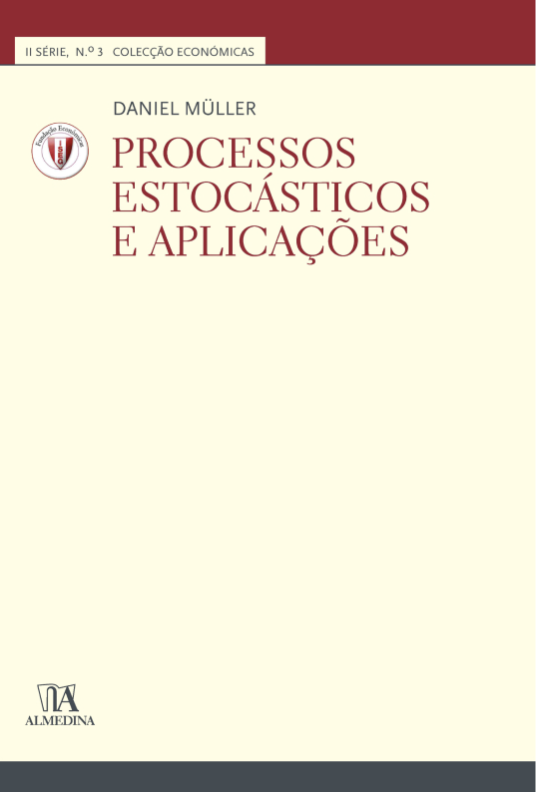
\includegraphics[width=0.2\linewidth]{figures/book1} \end{center}

\textbf{Secundária}

\begin{itemize}
\tightlist
\item
  Muller, D. (2011) Probabilidades e Processos Estocásticos. II Série, nº17, Coleção Económicas. Almedina.
\end{itemize}

\begin{center}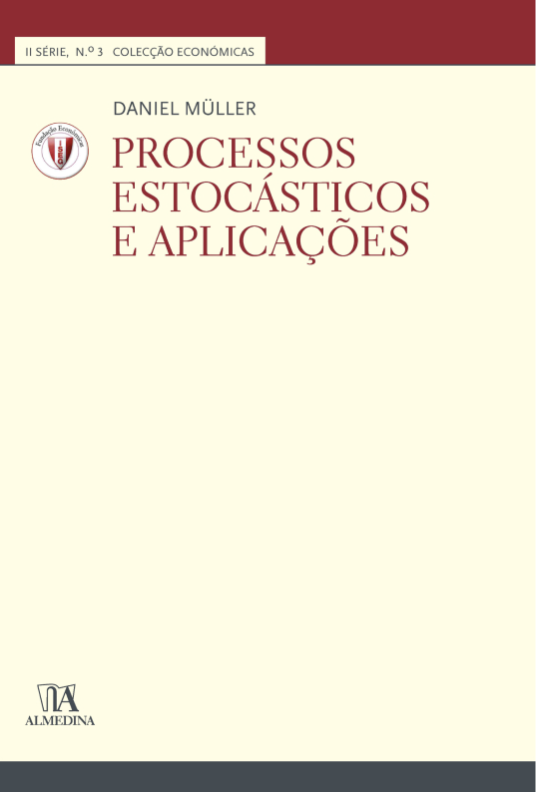
\includegraphics[width=0.2\linewidth]{figures/book1} \end{center}

\begin{itemize}
\tightlist
\item
  Taylor, H. M., Karlin, S. (1998) An Introduction to Stochastic Modeling (3rd Edition), Academic Press, New York.
\end{itemize}

\begin{center}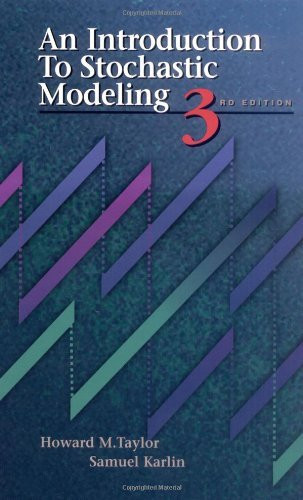
\includegraphics[width=0.2\linewidth]{figures/book3} \end{center}

\vfill

\(\,\)

\(\,\)

\(\,\)

\(\,\)

\textbf{Todos os direitos reservados. Nenhuma parte do conteúdo deste sítio pode ser reproduzida
ou distribuída sem a autorização prévia por escrito do autor. Sem autorização prévia por
escrito, não é permitido copiar ou reproduzir o texto, código e imagens.}

2025 \textbar{} Nuno M. Brites \textbar{}
\href{mailto:nbrites@iseg.ulisboa.pt}{\nolinkurl{nbrites@iseg.ulisboa.pt}}

\end{document}
